  %==============================================================================
% tento soubor pouzijte jako zaklad
% this file should be used as a base for the thesis
% (c) 2008 Michal Bidlo
% E-mail: bidlom AT fit vutbr cz
% Šablonu upravil / template edited by: Ing. Jaroslav Dytrych, dytrych@fit.vutbr.cz
%==============================================================================
% kodovaní: UTF-8 (zmena prikazem iconv, recode nebo cstocs)
% encoding: UTF-8 (you can change it by command iconv, recode or cstocs)
%------------------------------------------------------------------------------
% zpracování / processing: make, make pdf, make clean
%==============================================================================
% Soubory, které je nutné upravit: / Files which have to be edited:
%   xcoufa08-Pohled-na-stav-JUnit-pro-testovanou-instanci-eclipse-20-literatura-bibliography.bib - literatura / bibliography
%   xcoufa08-Pohled-na-stav-JUnit-pro-testovanou-instanci-eclipse-01-kapitoly-chapters.tex - obsah práce / the thesis content
%   xcoufa08-Pohled-na-stav-JUnit-pro-testovanou-instanci-eclipse-30-prilohy-appendices.tex - přílohy / appendices
%==============================================================================
%\documentclass[]{fitthesis} % bez zadání - pro začátek práce, aby nebyl problém s překladem
%\documentclass[english]{fitthesis} % without assignment - for the work start to avoid compilation problem
\documentclass[zadani]{fitthesis} % odevzdani do wisu - odkazy jsou barevné
%\documentclass[english,zadani]{fitthesis} % for submission to the IS FIT - links are color
%\documentclass[zadani,print]{fitthesis} % pro tisk - odkazy jsou černé
%\documentclass[english,zadani,print]{fitthesis} % for the print - links are black
% * Je-li prace psana v anglickem jazyce, je zapotrebi u tridy pouzit 
%   parametr english nasledovne:
%   If thesis is written in english, it is necessary to use 
%   parameter english as follows:
%      \documentclass[english]{fitthesis}
% * Je-li prace psana ve slovenskem jazyce, je zapotrebi u tridy pouzit 
%   parametr slovak nasledovne:
%      \documentclass[slovak]{fitthesis}

% Základní balíčky jsou dole v souboru šablony fitthesis.cls
% Basic packages are at the bottom of template file fitthesis.cls
%zde muzeme vlozit vlastni balicky / you can place own packages here
\usepackage[export]{adjustbox}
%\usepackage{enumitem}
%---rm---------------
\renewcommand{\rmdefault}{lmr}%zavede Latin Modern Roman jako rm / set Latin Modern Roman as rm
%---sf---------------
\renewcommand{\sfdefault}{qhv}%zavede TeX Gyre Heros jako sf
%---tt------------
\renewcommand{\ttdefault}{lmtt}% zavede Latin Modern tt jako tt

% vypne funkci šablony, která automaticky nahrazuje uvozovky,
% aby nebyly prováděny nevhodné náhrady v popisech API apod.
% disables function of the template which replaces quotation marks
% to avoid unnecessary replacements in the API descriptions etc.
\csdoublequotesoff

% =======================================================================
% balíček "hyperref" vytváří klikací odkazy v pdf, pokud tedy použijeme pdflatex
% problém je, že balíček hyperref musí být uveden jako poslední, takže nemůže
% být v šabloně
% "hyperref" package create clickable links in pdf if you are using pdflatex.
% Problem is that this package have to be introduced as the last one so it 
% can not be placed in the template file.
\ifWis
\ifx\pdfoutput\undefined % nejedeme pod pdflatexem / we are not using pdflatex
\else
  \usepackage{color}
  \usepackage[unicode,colorlinks,hyperindex,plainpages=false,pdftex]{hyperref}
  \definecolor{links}{rgb}{0.4,0.5,0}
  \definecolor{anchors}{rgb}{1,0,0}
  \def\AnchorColor{anchors}
  \def\LinkColor{links}
  \def\pdfBorderAttrs{/Border [0 0 0] }  % bez okrajů kolem odkazů / without margins around links
  \pdfcompresslevel=9
\fi
\else % pro tisk budou odkazy, na které se dá klikat, černé / for the print clickable links will be black
\ifx\pdfoutput\undefined % nejedeme pod pdflatexem / we are not using pdflatex
\else
  \usepackage{color}
  \usepackage[unicode,colorlinks,hyperindex,plainpages=false,pdftex,urlcolor=black,linkcolor=black,citecolor=black]{hyperref}
  \definecolor{links}{rgb}{0,0,0}
  \definecolor{anchors}{rgb}{0,0,0}
  \def\AnchorColor{anchors}
  \def\LinkColor{links}
  \def\pdfBorderAttrs{/Border [0 0 0] } % bez okrajů kolem odkazů / without margins around links
  \pdfcompresslevel=9
\fi
\fi
% Řešení problému, kdy klikací odkazy na obrázky vedou za obrázek
% This solves the problems with links which leads after the picture
\usepackage[all]{hypcap}

% Informace o práci/projektu / Information about the thesis
%---------------------------------------------------------------------------
\projectinfo{
  %Prace / Thesis
  project=BP,            %typ prace BP/SP/DP/DR  / thesis type (SP = term project)
  year=2017,             %rok odevzdání / year of submission
  date=\today,           %datum odevzdani / submission date
  %Nazev prace / thesis title
  title.cs={Pohled na stav JUnit pro testovanou instanci Eclipse},  %nazev prace v cestine ci slovenstine (dle zadani) / thesis title in czech language (according to assignment)
  title.en={JUnit Status View for Tested Eclipse Instance}, %nazev prace v anglictine / thesis title in english
  %Autor / Author
  author={Martin Coufal},   %cele jmeno a prijmeni autora / full name and surname of the author
  author.name={Martin},   %jmeno autora (pro citaci) / author name (for reference) 
  author.surname={Coufal},   %prijmeni autora (pro citaci) / author surname (for reference) 
  %author.title.p=Bc., %titul pred jmenem (nepovinne) / title before the name (optional)
  %author.title.a=PhD, %titul za jmenem (nepovinne) / title after the name (optional)
  %Ustav / Department
  department=UIFS, % doplnte prislusnou zkratku dle ustavu na zadani: UPSY/UIFS/UITS/UPGM
  %                  fill in appropriate abbreviation of the department according to assignment: UPSY/UIFS/UITS/UPGM
  %Skolitel / supervisor
  supervisor=Zbyněk Křivka, %cele jmeno a prijmeni skolitele / full name and surname of the supervisor
  supervisor.name={Zbyněk},   %jmeno skolitele (pro citaci) / supervisor name (for reference) 
  supervisor.surname={Křivka},   %prijmeni skolitele (pro citaci) / supervisor surname (for reference) 
  supervisor.title.p=Ing.,   %titul pred jmenem (nepovinne) / title before the name (optional)
  supervisor.title.a={Ph.D.},    %titul za jmenem (nepovinne) / title after the name (optional)
  %Klicova slova, abstrakty, prohlaseni a podekovani je mozne definovat 
  %bud pomoci nasledujicich parametru nebo pomoci vyhrazenych maker (viz dale)
  %Keywords, abstracts, declaration and acknowledgement can be defined by following 
  %parameters or using dedicated macros (see below)
  %===========================================================================
  %Klicova slova / keywords
  %keywords.cs={Klíčová slova v českém jazyce.}, %klicova slova v ceskem ci slovenskem jazyce
  %                                              keywords in czech or slovak language
  %keywords.en={Klíčová slova v anglickém jazyce.}, %klicova slova v anglickem jazyce / keywords in english
  %Abstract
  %abstract.cs={Výtah (abstrakt) práce v českém jazyce.}, % abstrakt v ceskem ci slovenskem jazyce
  %                                                         abstract in czech or slovak language
  %abstract.en={Výtah (abstrakt) práce v anglickém jazyce.}, % abstrakt v anglickem jazyce / abstract in english
  %Prohlaseni / Declaration
  %declaration={Prohlašuji, že jsem tuto bakalářskou práci vypracoval samostatně pod vedením pana ...},
  %Podekovani (nepovinne) / Acknowledgement (optional)
  %acknowledgment={Zde je možné uvést poděkování vedoucímu práce a těm, kteří poskytli odbornou pomoc.} % nepovinne
  %acknowledgment={Here it is possible to express thanks to the supervisor and to the people which provided professional help.} % optional
}

%Abstrakt (cesky, slovensky ci anglicky) / Abstract (in czech, slovak or english)
\abstract[cs]{
Cílem této práce je především návrh a implementace nástrojů umožňujících zobrazovat stav průběhu testů testované instance vývojového prostředí Eclipse. Řeší tak problém zobrazení výsledků právě probíhajících testů grafického uživatelského rozhraní, a to i při běhu na vzdálených platformách. Práce také obsahuje popis struktury vývojového prostředí Eclipse IDE\,(\emph{Integrated Development Environment}) a  popis nástroje JUnit, který je k implementaci zmíněných nástrojů využit.
Zobrazení potřebných výsledků uživateli je dosaženo pomocí dvou implementovaných aplikací. První je zásuvný modul pro vývojové prostředí Eclipse, který zjišťuje stav probíhajícího testování a zároveň zastává funkci serveru pro posílání potřebných informací připojeným klientům. Druhá aplikace slouží jako klient přijímající informace ze serveru. Tyto informace zpracovává a zobrazuje je do okna uživateli.
\todo{Jaké jsou konkrétní výsledky? Jak dobře je problém vyřešen?}
\todo{Čím je to užitečné vědě/čtenáři?}
Při testování grafického uživatelského rozhraní hraje roli spousta proměnných. Často jen změna komponenty nebo konfigurace platformy, na které testujeme, může způsobit selhání testu. Tento nástroj umožňuje detailnější pohled na probíhající testy. To může být užitečné jak v případě vytváření testů, tak v případě analýzy již hotových testů\,--\,lze snáze odhalit v jakém místě by se mohla nacházet chyba.
}

\abstract[en]{
Aim of this paper is design and implementation of tools which allow to display testing progress of Eclipse instance. This resolves problem of viewing currently running graphical user interface test results, even when running tests on a remote platforms. This thesis also contains description of Eclipse IDE\,(\emph{Integrated Development Environment}) and JUnit architecture. 
Displaying results to end user is achieved by implementing two separate applications. First one is Eclipse plug-in that collects test run information and creates server to send those information to all connected clients. Second application is used to display results of a test run. Results are received by client part of the application.
\todo{dopsat az bude hotove v CJ}
Automatic graphical user interface testing may be very fragile and it depends on various aspects. Even little change in component or platform configuration can lead to a test failure. Implemented applications allow to take a closer look at currently running tests. That is useful to locate error both when creating a new test or analysing already implemented one.
}

%Klicova slova (cesky, slovensky ci anglicky) / Keywords (in czech, slovak or english)
\keywords[cs]{zásuvný modul pro Eclipse, testování Eclipse, rozšíření pro JUnit, výsledky JUnit, \todo{...}}
\keywords[en]{Eclipse plug-in, Eclipse testing, JUnit extension, JUnit results, \todo{...}}

%Prohlaseni (u anglicky psane prace anglicky, u slovensky psane prace slovensky)
%Declaration (for thesis in english should be in english)
\declaration{Prohlašuji, že jsem tuto bakalářskou práci vypracoval samostatně pod vedením pana Ing. Zbyňka Křivky, Ph.D.
Další informace mi poskytl Ing. Pavol Srna, zaměstnanec firmy Red Hat Czech s.r.o., zabývající se testováním vývojového prostředí Eclipse.
Uvedl jsem všechny literární prameny a publikace, ze kterých jsem čerpal.}

% \declaration{Hereby I declare that this bachelor's thesis was prepared as an original author’s work under the supervision of Mr. X
% The supplementary information was provided by Mr. Y
% All the relevant information sources, which were used during preparation of this thesis, are properly cited and included in the list of references.}

%Podekovani (nepovinne, nejlepe v jazyce prace) / Acknowledgement (optional, ideally in the language of the thesis)
\acknowledgment{\todo{V této sekci je možno uvést poděkování vedoucímu práce a těm, kteří poskytli odbornou pomoc
(externí zadavatel, konzultant, apod.).}}
%\acknowledgment{Here it is possible to express thanks to the supervisor and to the people which provided professional help
%(external submitter, consultant, etc.).}

% řeší první/poslední řádek odstavce na předchozí/následující stránce
% solves first/last row of the paragraph on the previous/next page
\clubpenalty=10000
\widowpenalty=10000

\begin{document}
  % Vysazeni titulnich stran / Typesetting of the title pages
  % ----------------------------------------------
  \maketitle
  % Obsah
  % ----------------------------------------------
  \tableofcontents
  
  % Seznam obrazku a tabulek (pokud prace obsahuje velke mnozstvi obrazku, tak se to hodi)
  % List of figures and list of tables (if the thesis contains a lot of pictures, it is good)
\ifczech
  \renewcommand\listfigurename{Seznam obrázků}
\fi
\ifslovak
  \renewcommand\listfigurename{Zoznam obrázkov}
\fi

  % \listoffigures
\ifczech
  \renewcommand\listtablename{Seznam tabulek}
\fi
\ifslovak
  \renewcommand\listtablename{Zoznam tabuliek}
\fi

  % \listoftables 

  % vynechani stranky v oboustrannem rezimu
  % Skip the page in the two-sided mode
  \iftwoside
    \cleardoublepage
  \fi

  % Text prace / Thesis text
  % ----------------------------------------------
  %=========================================================================%
% KAPITOLA 1: Ú V O D                                                     %
\chapter{Úvod}                                                            %
%=========================================================================%
V~dnešní době se na testování klade velký důraz, a proto je potřeba se touto částí vývoje software zabývat detailně. Aplikace lze testovat různými způsoby, od jednoduchých manuálních testů po sofistikované nástroje automaticky spouštějící vybrané sady testů. Pro tyto účely existuje mnoho nástrojů\footnote{\url{https://en.wikipedia.org/wiki/List_of_unit_testing_frameworks}}, které usnadňují programátorům práci. Cílem těchto nástrojů je redukce množství napsaného kódu opakujícího se v~testech pro podobné komponenty nebo jejich vlastnosti.

Co se týče programovacího jazyka Java, můžeme vybírat z~velkého množství nástrojů\footnote{\url{https://en.wikipedia.org/wiki/List_of_unit_testing_frameworks\#Java}} pro testování podle toho, jaký aspekt software chceme testovat. Pro testování Servler, Bean a Java tříd lze testovat pomocí nástrojů jako jsou například \emph{Servlets}, \emph{JUnit}, \emph{Arquillian}, \emph{ServletUnit} nebo \emph{Mock objects}. Pro testování grafického uživatelského rozhraní vytvořeného pomocí Swing lze použít například \emph{UISpec4j}, \emph{Abbot}, \emph{Fest}, \emph{QF-Test} a další. Pro funkcionální testování lze použít například \emph{HTTPUnit}, \emph{JWebUnit}, \emph{TestNG} nebo \emph{Selenium Webdriver}, zatímco pro výkonnostní testování lze použít například \emph{Apache JMeter} \cite{softwaretestinghelp}.

Tato práce se zabývá popisem infrastruktury vývojového prostředí \emph{Eclipse} (dále zkráceně Eclipse IDE) a jeho zásuvných modulů s~přihlédnutím k~budoucímu použití pro vytvoření vlastního zásuvného modulu. Dále se zabývá popisem testovacího rámce JUnit a jeho architekturou. JUnit je snadno rozšiřitelný a je obsažen ve velkém množství testovacích nástrojů a vývojových prostředí včetně Eclipse IDE, kde ho lze použít při testování jeho grafického uživatelského rozhraní (dále zkráceně GUI). Klíčovou částí práce je návrh a implementace zásuvného modulu Eclipse IDE, který zpracovává data z~testovacího rámce JUnit a posílá informace o~průběhu testů do klientské aplikace, kde je zobrazuje uživateli. Důvodem pro tvorbu tohoto projektu je potřeba programátora zjistit v~jaké fázi se probíhající sada testů nachází, který test v~dané chvíli běží a jak dopadly již proběhlé testy.

  %=========================================================================%
% KAPITOLA 2: V Ý V O J O V É - P R O S T Ř E D Í - E C L I P S E         %
\chapter{Vývojové prostředí Eclipse}                                      %
\label{chapter:eclipse_ide}
%=========================================================================%
Eclipse IDE je integrované vývojové prostředí poskytující podporu pro mnoho programovacích jazyků, jako jsou například Java, C, C++, JavaScript a PHP.  Je záložen na modulové architektuře, která umožňuje snadné rozšíření této platformy. Pro přidání nové funkcionality do vývojového prostředí stačí nainstalovat příslušný zásuvný modul (\emph{angl. plug-in}). Projekt Eclipse je udržován radou správců \emph{eclipse.org}, která vznikla z~iniciativy společností \emph{Borland}, \emph{IBM}, \emph{MERANT}, \emph{QNX Software Systems}, \emph{Rational Software}, \emph{Red Hat}, \emph{SuSE}, \emph{TogetherSoft} a \emph{Webgain}. Cílem eclipse.org je tvorba univerzálního rozšiřitelného integrovaného vývojového prostředí, které poskytuje nástroje pro integraci různých platforem a zároveň potřebné nástroje pro jejich tvorbu a rozšíření \cite{eclipse-org}.

V~následující kapitole je popsána struktura Eclipse IDE a částí, ze kterých se skládá. Dále je zde popsán systém zásuvných modulů Eclipse IDE a jejich částí.

  \section{Infrastruktura Eclipse IDE}
  \label{section:Infrastruktura_Eclipse_IDE}
  %===============================
  Eclipse IDE není monolitické vývojové prostředí, ale spíše komplexní soubor zásuvných modulů. V~základě je rozdělen do několika podsystémů, které jsou koncipovány jako jeden nebo více zásuvných modulů. Minimální množina zásuvných modulů, která je potřeba pro vývoj klientské aplikace se nazývá \emph{Eclipse RCP} (\emph{Rich Client Platform})\footnote{\url{https://wiki.eclipse.org/Rich_Client_Platform}}. V~dnešní době se však Eclipse IDE často používá i pro vývoj serverových aplikací, tato infrastruktura se potom nazývá \emph{EAF} (\emph{Eclipse Aplication Framework}). Důležitou komponentou je jádro, které načítá jednotlivé zásuvné moduly. Toto jádro je implementováno na základě specifikace \emph{OSGi Service Platform}, která definuje standard pro dynamické modulární systémy v~Javě \cite{Plugins}. Tento standard je definován mezinárodním konsorciem \emph{OSGi Alliance}\footnote{\url{https://www.osgi.org/}}. Díky implementaci rámce \emph{OSGi Equinox}\footnote{\url{http://www.eclipse.org/equinox/}} používá Eclipse IDE pro načítání jednotlivých zásuvných modulů návrhový vzor \emph{lazy-loading}, který zajišťuje načítání jen nezbytných zásuvných modulů.
  \\
  \\
  \noindent
  Zásuvné moduly se v~základu dělí podle funkce do několika skupin \cite{Plugins}:
  \begin{description}
    \item[Core:] skupina nízkoúrovňových zásuvných modulů zajišťujících základní funkce jako jsou zpracování rozšíření zásuvných modulů a zdrojových kódů.
    \item[SWT\,(Standard Widget Toolkit):] knihovna nástrojů pro manipulaci s~uživatelským rozhraním, která poskytuje API nezávislé na operačním systému.
    \item[JFace:] knihovna přidávající další funkcionalitu jako nástavbu k~SWT.
    \item[GEF:] rámec poskytující prostředí pro vývoj grafických editorů.
    \item[Workbench:] skupina zásuvných modulů poskytujících funkcionalitu specifickou přímo pro Eclipse IDE, jako je manipulace s~projekty nebo grafickými prvky (pohledy, perspektivami, atd.).
    \item[Team:] skupina zásuvných modulů poskytujících podporu pro správu verzí v~Eclipse IDE.
    \item[Help:] poskytuje dokumentaci k~jednotlivým prvkům Eclipse IDE.
    \item[JDT\,(Java Development Tools)\footnotemark:] \footnotetext{\url{http://www.eclipse.org/jdt/}} přidává podporu pro vývoj Java aplikací a navíc do Eclipse IDE přidává perspektivy, pohledy, průvodce a další nástroje pro práci s~Javou.
    \item[PDE\,(Plug-in Development Enviroment)\footnotemark:] \footnotetext{\url{http://www.eclipse.org/pde/}} skupina zásuvných modulů poskytujících různé nástroje\,(pohledy, editory, atd.) pro práci se zásuvnými moduly a jejich manifesty.
    \item[Mylyn:] poskytuje uživatelské rozhraní pro správu a prezentaci informací definovaných uživatelem.
  \end{description}

  \begin{figure}
    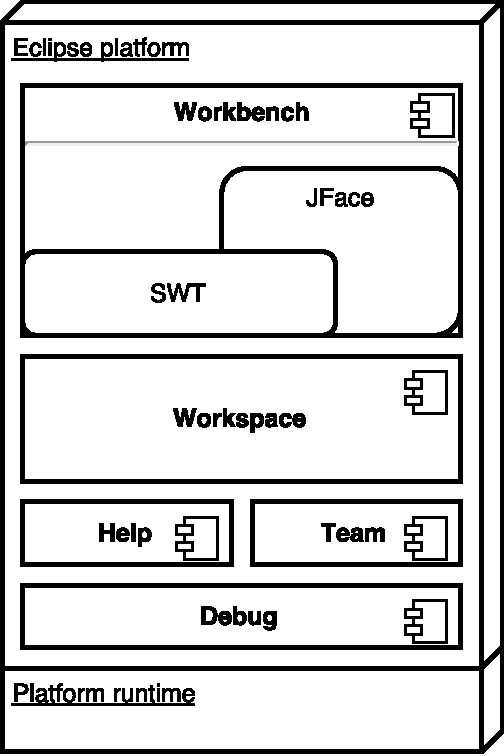
\includegraphics[width=0.5\textwidth, center]{obrazky-figures/eclipse_arch.pdf}
    \caption[Architektura platformy Eclipse.]{Architektura platformy Eclipse (inspirováno v~\cite{eclipse-platform}).}
    \label{fig:eclipse_arch}
  \end{figure}

  Na obrázku \ref{fig:eclipse_arch} jsou znázorněny základní komponenty platformy Eclipse. \emph{Workbench} představuje obálku, která umožňuje uživateli orientaci ve vývojovém prostředí. Definuje \emph{body rozšíření}\,(\emph{angl. extension points}), kde je možno k~zásuvnému modulu přidat další, rozšiřující modul. Díky těmto bodům lze přidávat například komponenty grafického rozhraní, jako jsou pohledy, editory a menu. \emph{Pracovní plocha}\,(\emph{angl. Workspace}) definuje rozhraní pro programování aplikací\,(dále zkráceně API) za účelem vytváření a správy projektů, souborů a složek. Zde jsou projekty překládány a sestavovány. Pracovní plocha navíc obsahuje další informace k~projektům, jako je například uživatelské nastavení. \emph{Help} poskytuje body rozšíření sloužící pro zobrazení nápovědy nebo dokumentace. Modul \emph{Team} definuje model pro vývoj aplikací v~týmu, s~podporou správy verzí aplikace a zdrojových kódů. Komponenta \emph{Platform Runtime} spravuje informace týkající se právě běžícího prostředí Eclipse. Například dynamicky vyhledává a spravuje informace o~zásuvných modulech a jejich bodech rozšíření. Také poskytuje informace ohledně správy procesů, argumentů příkazové řádky, adresářové struktury jednotlivých zdrojů a další \cite{Plugins}.

    \subsection{Workbench}
    %*********************
    Termín Workbench odkazuje na desktopové vývojové prostředí. Jeho cílem je integrace různých nástrojů a poskytnutí základního schématu pro tvorbu, správu a navigaci ve zdrojích pracovní plochy. Běžně se ve Workbench nachází lišta s~hlavním menu, nástrojová lišta a několik pohledů, případně editorů \cite{eclipse-workbench}. Grafické prvky vývojového prostředí jsou však pro uživatele přizpůsobitelné. Běžný vzhled Eclipse Workbench je zobrazen na obrázku \ref{fig:eclipse_workbench}.

    \begin{figure}
      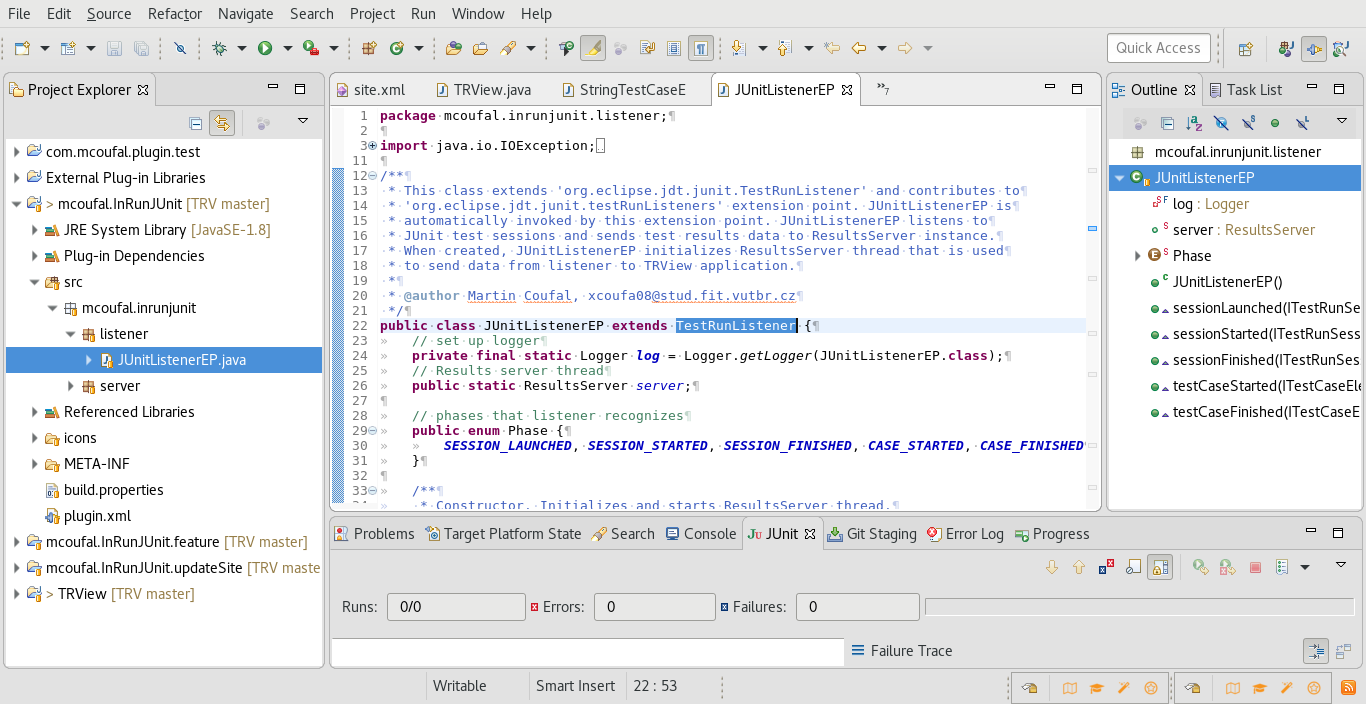
\includegraphics[width=\textwidth, keepaspectratio, center]{obrazky-figures/eclipse_workbench.png}
      \caption{Běžný vzhled Eclipse Workbench.}
      \label{fig:eclipse_workbench}
    \end{figure}

      \subsubsection{Pohledy}
      %----------------------
      Pohled je jednou ze základních komponent tvořících grafické uživatelské rozhraní Eclipse IDE. Slouží k~zobrazování informací uživateli a také k~navigaci ve vývojovém prostředí. Každý pohled může mít svá menu a své nástrojové lišty.

      Pro vytvoření nového pohledu je zapotřebí dvou kroků\,--\,vytvoření kategorie pohledu\,(pokud ho nechceme vytvořit v~některé z~již existujících kategorií) a deklarace nového pohledu. Obě dvě změny probíhají v~manifestu zásuvného modulu. Přesto, že je možné tyto změny do manifestu dopsat ručně, vývojové prostředí Eclipse nabízí praktické nástroje pro editaci manifestů zásuvných modulů. Otevření některého z~manifestů zásuvného modulu spustí editor zásuvného modulu. Nastavení rozšíření zásuvného modulu lze upravovat v~záložce \emph{Extensions}. Pro přidání kategorie pohledu i deklarace pohledu samotného je nutné nejdříve přidat správný bod rozšíření. Všechny pohledy se připojují na bod rozšíření \texttt{org.eclipse.ui.views}. K~tomuto bodu rozšíření lze přidat novou kategorii pohledu, nebo deklarovat nový pohled.

      Běžně používanou třídou implementující toto rozhraní je \texttt{org.eclipse.ui.part.ViewPart}. Zdrojový kód s~popisem chování daného pohledu se nachází ve třídě implementující rozhraní \texttt{org.eclipse.ui.IViewPart} \cite{Plugins}.

      \subsubsection{Perspektivy}
      %--------------------------
      Perspektivy slouží jako nástroj pro seskupení relevantních komponent v~aktivním okně Workbench. Komponenty se seskupují podle úkonu, který bude uživatel vykonávat a  zároveň podle programovacího jazyka, ve kterém uživatel projekt vytváří. Eclipse IDE umožňuje přidání nových perspektiv pomocí zásuvných modulů a bodů rozšíření. Pokud je to žádoucí, lze také při přidání nového zásuvného modulu některou z~již existujících perspektiv pouze upravit.

      Pro přidání nové perspektivy, podobně jako u~přidání nového pohledu, je nutno do manifestu zásuvného modulu přidat správný bod rozšíření\,--\,\texttt{org.eclipse.ui.perspectives}. Rozložení komponent v~dané perspektivě je definováno ve třídě implementující rozhraní \texttt{IPerspectiveFactory} \cite{Plugins}. Přidat nové rozšíření zásuvného modulu implementující novou nebo upravenou perspektivu lze jednoduše pomocí nástrojů v~záložce \emph{Extensions} u~editoru zásuvného modulu. Chceme-li perspektivu pouze upravit, lze při tvorbě nové perspektivy vybrat některou z~již existujících.

      \subsubsection{Editory}
      %----------------------
      Editory slouží jako hlavní nástroj pro úpravu zdrojového kódu a jiných textových souborů. Eclipse IDE nabízí mnoho editorů, které je možno nainstalovat v~rámci nějakého ze zásuvných modulů. Nejzákladnějším editorem je textový editor. Ten poskytuje pouze základní funkce pro práci s~textem a neposkytuje možnost zvýraznění syntaxe nebo její kontrolu. I~základní textový editor je však možno dále rozšířit pomocí dalších zásuvných modulů.

      Editor lze přidat pomocí rozšiřujícího bodu \texttt{org.eclipse.ui.editors}. Na ten lze připojit vlastní třídu implementující rozhraní \texttt{org.eclipse.ui.IEditorPart} \cite{Plugins}. Proces vytváření nového editoru je stejný jako v~předchozích dvou případech.

      \subsection{Standard Widget Toolkit}
      %***********************************
      SWT představuje tenkou vrstvu nad nativním ovládáním uživatelského rozhraní platformy Eclipse. Poskytuje tak rozhraní pro pohodlnější interakci s~uživatelským rozhraním, které zahrnuje většinu prvků nacházejících se v~platformě Eclipse a tak lze pomocí SWT snadno vytvářet aplikace s~grafickým uživatelským rozhraním \cite{Plugins}. Zároveň je na SWT postaven zásuvný modul \emph{SWTBot}, sloužící pro testování uživatelského rozhraní.

  \section{Architektura zásuvných modulů v~Eclipse IDE}
  %====================================================
  Každý zásuvný modul v~Eclipse IDE slouží buď jako knihovna pro dodatečné funkce jiným zásuvným modulům, nebo pro rozšíření funkcionality platformy. Chování každého zásuvného modulu je popsáno v~jeho zdrojovém kódu. Závislosti, body rozšíření a služby poskytované  zásuvným modulem jsou popsány v~manifestech zásuvného modulu\,--\,souborech \texttt{MANIFEST.MF} a \texttt{plugin.xml}. Načítání nových zásuvných modulů probíhá až když je modul přímo vyžadován\,(dle návrhového vzoru lazy-loading). Na začátku jsou načteny pouze manifesty zásuvných modulů. Ty poskytují základní informace o~zásuvném modulu a nemusí se tak načítat kompletní zásuvný modul. Díky tomuto modelu je Eclipse IDE i přes velké množství možných instalovaných zásuvných modulů kompaktnější a výrazně rychlejší při startu.

  Zásuvný modul\,(ať už v~podobě Java archivu JAR nebo v~podobě adresáře projektu) se skládá z~Javových tříd, manifestů zásuvného modulu\,(\texttt{MANIFEST.MF} a \texttt{plugin.xml}) a obrázkových souborů, které jsou typicky umístěny v~adresářích pojmenovaných \emph{icons} nebo \emph{images}. Pokud je zásuvný modul ve formě adresáře, archiv JAR je uložen v~některém z~podadresářů. Název archivu JAR a jeho umístění je v~takovém případě definováno v~souboru \texttt{MANIFEST.MF}.

    \subsection{Model zásuvných modulů}
    %********************************
    Eclipse IDE při startu prohledá všechny adresáře se zásuvnými moduly a vytvoří vlastní model obsahující každý nalezený zásuvný modul. Tento model se vytváří pomocí manifestů zásuvných modulů tak, aby Elipse nemusel načítat celé zásuvné modely a ušetřil tak čas a místo. Informace o~jednotlivých nainstalovaných zásuvných modulech jsou uloženy v~balíčcích\,(\emph{angl. bundles}). Získáváním informací přes rozhraní těchto balíčků zajistíme, aby se zásuvné moduly nenačítaly, dokud nejsou opravdu zapotřebí.

    Původně mělo Eclipse IDE vlastní mechanismus pro běh aplikace, ale to znemožnilo použití již vytvořených technologií v~jiných oblastech jako Avalon\footnote{\url{https://avalon.apache.org}} nebo JMX\footnote{\url{http://www.oracle.com/technetwork/articles/java/javamanagement-140525.html}}. Proto byl nakonec nahrazen mechanismem pro běh aplikace založeném na technologii OSGi Alliance, která poskytuje model s~detailní specifikací a podporuje dynamické chování \cite{Plugins}.

    \subsection{Manifesty zásuvného modulu}
    %**************************************
    Manifesty zásuvného modulu jsou dva soubory\,--\,\texttt{MANIFEST.MF} a \texttt{plugin.xml}. První zmíněný obsahuje data nutná pro běh zásuvného modulu jako jsou \emph{identifikátor}, \emph{verze} a \emph{závislosti} zásuvného modulu. Druhý obsahuje data ve formátu XML popisující případná rozšíření a body rozšíření.

      \subsubsection{Soubor `MANIFEST.MF'}
      %-------------------------------------
      V~každém souboru \texttt{MANIFEST.MF} zásuvného modulu se nacházejí záznamy pro jméno, identifikátor, verzi, spouštěč a poskytovatele balíčku zásuvného modulu. Dále se zde mohou vyskytovat záznamy s~cestou k~knihovnám\,(\emph{ClassPath}), exportovanými balíčky a závislostmi zásuvného modulu.

      Jméno\,(\emph{Bundle-Name}) a poskytovatel\,(\emph{Bundle-Vendor}) jsou \emph{human-readable}\footnote{\url{https://en.oxforddictionaries.com/definition/us/human-readable}} řetězce, které nemusí být unikátní a lze je ukládat do zvláštního souboru \texttt{plugin.properties} za účelem internacionalizace.

      Identifikátor\,(\emph{Bundle-SymbolicName}) slouží k~jednoznačné identifikaci daného balíčku. Většinou se jako identifikátor balíčku používá Javová konvence pro pojmenování balíčků: \texttt{com.<název společnosti>.<komponenta>[.<část komponenty>]}, kde část dané komponenty\,(například '\texttt{ui}' nebo '\texttt{core}') se uvádí v~případě větších komponent, kde jsou jednotlivé balíčky rozděleny.

      Verze\,(\emph{Bundle-Version}) slouží k~jednoznačné identifikaci verze daného balíčku. V~případě shody identifikátorů je vždy vybrán balíček s~novějším číslem verze. Toto číslo se skládá ze 3 číslic oddělených tečkami a v~případě potřeby i alfanumerického řetězce použitelného pro užší specifikaci\,(například '\texttt{1.2.3.beta}'). První číslo označuje majoritní verzi produktu, druhé minoritní verzi produktu a třetí slouží k~označení úrovně služeb\footnote{více k~číslování balíčků lze nalézt na \url{https://wiki.eclipse.org/Version_Numbering}}.

      Spouštěč\,(\emph{Bundle-Activator}) je volitelná část manifestu která umožňuje specifikovat třídu implementující rozhraní \texttt{BundleActivator} a poskytuje tak metody \texttt{start()} a \texttt{stop()}, které jsou přínosné pro správu životního cyklu balíčku.

      Cesta k~knihovnám\,(\emph{Bundle-ClassPath}) je čárkami oddělený seznam knihoven ve formátu JAR obsahujících zdrojový kód zásuvného modulu.

      Záznam s~exportovanými balíčky\,(\emph{Export-Package}) je podmnožina z~cesty k~knihovnám obsahující ty knihovny, které se mají exportovat, aby byly viditelné pro ostatní zásuvné moduly.

      Eclipse IDE vytváří pro každý načtený zásuvný modul novou instanci, která slouží k~vyhledávání a načítání zásuvných modulů a používá \emph{záznam závislostí} v~manifestu k~určení viditelnosti ostatních zásuvných modulů. Záznam závislostí\,(\emph{Require-Bundle}) je seznam zásuvných modulů, které jsou pro daný zásuvný modul viditelné z~hlediska vykonávání programu \cite{Plugins}.

      \subsubsection{Soubor `plugin.xml'}
      %------------------------------------
      V~tomto manifestu zásuvného modulu mohou být uvedeny body rozšíření, na které je možno připojit nový zásuvný modul rozšiřující stávající funkcionalitu. Toto odloučení od rozšiřujících zásuvných modulů umožňuje existenci základního zásuvného modulu bez znalosti jakýchkoliv informací o~ostatních zásuvných modulech. To zajišťuje snazší spolupráci při implementaci a znovupoužitelnost již implementovaných částí \cite{Plugins}. Bod rozšíření obvykle definuje identifikátor, jméno a schéma\,(viz obrázek \ref{code:extension_point_declaration}). Schéma určuje, co musí rozšiřující zásuvný modul splnit pro správné rozšíření tohoto zásuvného modulu. Deklarace bodu rozšíření se vkládá do bloku s~označením \texttt{<plugin>}. 

      \lstset{language=xml}
      \begin{figure}
	\begin{lstlisting}[frame=single]
<extension-point id="org.example.extensionpoints.point"
  name="Point"
  schema="schemas/scheme.exsd" />
	\end{lstlisting}
	\caption{Příklad zdrojového kódu s~definicí bodu rozšíření.}
	\label{code:extension_point_declaration}
      \end{figure}

      Dále je zde možno definovat, který zásuvný modul chceme stávajícím modulem rozšířit\,--\,k tomu slouží rozšíření zásuvného modulu\,(viz obrázek \ref{code:extension_declaration}). Obsah bloku \texttt{<extension point>} je dán bodem rozšíření na který se připojujeme. V~případě obrázku \ref{code:extension_declaration} jde o~připojení na bod rozšíření \texttt{org.eclipse.ui.views}, který umožňuje přidání vlastního pohledu. K~tomu je třeba specifikovat kategorii\,(v případě že vytváříme novou) a zároveň jednotlivé parametry implementovaného pohledu.

      \begin{figure}
	\begin{lstlisting}[frame=single]
<extension
  point="org.eclipse.ui.views">
  <category
    id="com.example.myview"
    name="Sample Category">
  </category>
  <view
    category="com.example.myview"
    class="com.example.myview.views.SampleView"
    icon="icons/sample.gif"
    id="com.example.myview.views.SampleView"
    name="Sample View">
  </view>
</extension>
	\end{lstlisting}
	\caption{Příklad zdrojového kódu s~připojením na bod rozšíření \texttt{org.eclipse.ui.views}.}
	\label{code:extension_declaration}
      \end{figure}
  %=========================================================================%
% - - - KAPITOLA 3: J U N I T                                             %
\chapter{Testovací rámec JUnit}                                           %
%=========================================================================%
JUnit je jednoduchý nástroj pro psaní testů a testování aplikací. Jeho vývoj je založen na otevřeném zdrojovém kódu (\emph{angl. open-source}), a proto lze najít další nástroje, které rámec JUnit používají nebo z~něj vycházejí. Cílem JUnit je poskytovat nástroj, který by umožňoval \todo{citace-tusim Beck - overit}:
\begin{description}
  \item[Jednoduchost psaní testů]
  Programátor nemusí psát zbytečně mnoho kódu, zbytek za něj vykoná rámec JUnit.
  \item[Snadné pochopení rámce JUnit]
  Rámec by měl být pro Javu přirozený, tak aby se programátor naučil s~rámcem pracovat co nejrychleji.
  \item[Rychlé provedení testů]
  Spouštění jednotlivých testovacích případů by mělo probíhat bez zbytečných odkladů tak, aby šetřilo programátorům čas.
  \item[Izolované provedení testů]
  Rámec by měl poskytovat izolaci jednotlivých testovacích případů, která zajišťuje dostatečnou stabilitu testovacích sad.
  \item[Skládat a provádět různé kombinace testů]
  Lze spustit například testy se stejným štítkem\,(\emph{angl. tag}) nebo jen vybrané testy v~sadě.
\end{description}

Bohužel jsou některé z~těchto podmínek v~rozporu mezi sebou a tak nelze splnit všechny z~těchto požadavků naplno. V~této kapitole je popsán testovací rámec JUnit, jeho architektura, aplikační rozhraní, vybraná existující rozšíření a zásuvné moduly postavené na tomto rámci. 


  \section{Architektura rámce JUnit}
  %=================================
  V~roce 1999 publikoval Kent Beck svůj rámec pro jednotkové testování pro programovací jazyk \emph{Smalltalk} -- SmalltalkUnit (zkráceně SUnit). Idea tohoto rámce spočívá v~nalezení ideální kombinace mezi jednoduchostí a užitečností. Později Erich Gamma přepsal SUnit do jazyka Java a vytvořil tak JUnit. Posléze tak začaly vznikat mnohé obdoby rámce JUnit podporující mnohé programovací jazyky \cite{UnitTestFrameworks}:
  
  \begin{description}
   \item[CppUnit:] pro jazyk C++
   \item[CUnit:] pro jazyk C
   \item[NUnit:] pro jazyk .NET, včetně C\#, VB.NET, J\# a Managed C++
   \item[PyUnit:] pro jayzk Python
   \item[vbUnit:] pro jazyk Visula Basic
   \item[utPLSQL:] pro jazyk PL/SQL od firmy Oracle
   \item[MinUnit:] minimalistická verze pro jazyk C
  \end{description}


    \subsection{xUnit}
    %*****************
    Všechny rámce založené na xUnit se drží stejných základů. Klíčovými třídami v~každém rámci jsou třídy TestCase, TestRunner, TestFixture, TestSuite a TestResult \cite{UnitTestFrameworks}.

    \begin{description}
      \item[TestCase] je základní třídou reprezentující jednotkový test. Všechny jednotkové testy jsou odvozeny od této třídy a dědí její vlastnosti.
      \item[TestRunner] je třída spouštějící jednotlivé testy a zpracovávající jednotlivé výsledky. Existují dva základní typy runnerů -- grafický a textový. Nejdůležitější metodou je metoda run(), která spouští runner a testy zadané jako parametr této metody.
      \item[TestFixture] 
      \item[TestSuite] asm sad 
      \item[TestResult] amskd mksa 
    \end{description}


    \subsection{JUnit}
    %*****************
    % Popis architektury / implementace JUnit 
    \todo{Lorem ipsum dolor sit amet} viz obr \ref{fig:junit_arch}.

    \todo{Lze vybírat spuštěné testy dle štítků?}
    
    \begin{figure}[!h]
      
\includegraphics[width=\textwidth, center]{obrazky-figures/placeholder.pdf}
      \caption{Architektura testovacího rámce JUnit.}
      \label{fig:junit_arch}
    \end{figure}


  \section{Rozhraní pro programování aplikací rámce JUnit}
  %=======================================================
  \todo{Lorem isusm dolor sit amet.}
    
    \subsection{Testovací třídy v~rámci JUnit}
    Testovací třída v~rámci Junit je třída obsahující jednotlivé testovací případy. Jednotlivé testovací případy jsou od ostatních metod odlišeny anotací \texttt{@Test} \cite{vogella:JUnit}. Díky tomu rámec JUnit pozná jednotlivé testy, které má spustit.
    
    \subsection{Testovací sady v~rámci JUnit}
    Díky vytváření testovacích sad lze seskupovat různé testovací třídy dle potřeby programátora. Testovací sada se definuje pomocí anotace \texttt{@SuiteClasses}. Jako parametr anotace je zadán seznam jednotlivých testovacích tříd, které do testovací sady patří. Spuštěním testovací sady se tak spustí všechny testovací třídy.
    \todo{Anotace RunWith - dopsat text + je nejaky implicitni runner, nebo je treba zadavat vzdy explicitne?}
    
    \subsection{Parametrizované testovací třídy}
    \todo{Lorem ipsum dolor sit amet.}
    
    \subsection{Přeskočení testovacího případu}
    \todo{Lorem ipsum dolor sit amet.}

  \section{Rozšíření rámce JUnit}
  %==============================
  \todo{Lorem ipsum dolor sit amet.}

  \section{Zásuvné moduly Eclipse IDE rozšiřující rámec JUnit}
  %===========================================================
  \todo{Lorem ipsum dolor sit amet.}
  % Zminit jake moduly rozsiruji JUnit a jak, detailneji popsat jen ten co pouziji.
    \subsection{Zásuvný modul org.junit.???}
    %***************************************
    \todo{Lorem ipsum dolor sit amet.}
    \subsubsection{JUnit ui}
    %-----------------------
    % Tady by mela byt popsana zakladni struktura daneho pluginu + Tridy dulezite z hlediska implementace 
    \todo{Lorem ipsum dolor sit amet.}
    \subsubsection{JUnit core}
    %-------------------------
    % Tady by mela byt popsana zakladni struktura daneho pluginu + Tridy dulezite z hlediska implementace
    \todo{Lorem ipsum dolor sit amet.}
  %=========================================================================%
% - - KAPITOLA 4: Z Á S U V N Ý - M O D U L - I n R u n J U n i t V i e w %
\chapter{Implementovaná aplikace TestRunView}                             %
%=========================================================================%
Díky architektuře zásuvných modulů je snadné rozšířit Eclipse IDE o novou funkcionalitu a tak poskytuje četné množství prvků, které je vhodné otestovat. V rámci testování GUI Eclipse IDE se používají rozsáhlé testovací sady testující velké množství aspektů a možností. Automatické testy GUI jsou ale časově náročné a nejsou dokonalé. Vzniká tak potřeba kontroly nad sadou s probíhajícími testy. Průběh testů lze sledovat pomocí zásuvného modulu \texttt{org.eclipse.jdt.junit}, který poskytuje pohled JUnit zobrazující potřebné informace o probíhajících testech. Navíc umožňuje znovu spustit testovací sadu a také si uchovává historii testovaných sad. Problémem tohoto pohledu je, že při spuštění testovací sady se otevírá nové okno s testovanou instancí Eclipse IDE. To způsobí překrytí pohledu JUnit a proto není možné sledovat tento pohled v průběhu testování. Také z hlediska časové náročnosti může být výhodnější testovat na vzdálených serverech a spouštět testy z terminálu. V takovém případě nelze pohled JUnit k zobrazení detailů o testování použít.

Implementovaná aplikace \emph{TestRunView} (dále zkráceně TRV) poskytuje možnost zobrazení informací o probíhajícím testování GUI Eclipse IDE bez narušení průběhu testů. Mezi důležité informace které tato aplikace zobrazuje patří zobrazení průběhu a výsledků jednotlivých testovacích případů v rámci spuštěné testovací sady. V případě nějaké chyby v testovací sadě potom lze lépe prozkoumat kde chyba nastala a jaká byla její příčina.

Tato kapitola detailně popisuje architekturu, implementaci, způsob testování a využití této aplikace.

  \section{Návrh architektury aplikace TestRunView}
  %================================================

  V rámci návrhu bylo třeba zvážit způsoby, jakými lze data o probíhajících testech získávat a jakými lze tyto data zobrazovat. Ve společnosti \emph{Red Hat} se používají pro testování rámce JUnit a \emph{RedDeer}\footnote{\url{https://github.com/jboss-reddeer}}. RedDeer je rámec pro testování zásuvných modulů Eclipse IDE a využívá k tomu rámec JUnit. Pomocí implementace vlastního \emph{runneru} dostává kontrolu nad probíhajícími testy. To umožňuje definovat například pořadí a typ spuštěných testů, nebo vytvářet vlastní anotace a tak definovat nové fáze probíhající v rámci testování.

  Data tedy lze získávat z obou zásuvných modulů\,--\,JUnitu i RedDeeru. JUnit ovšem narozdíl od RedDeeru poskytuje možnost připojit se pomocí bodu rozšíření\\\texttt{org.eclipse.jdt.junit.testRunListeners} a tak umožňuje širší použití výsledné aplikace. Vytvořený zásuvný modul není třeba explicitně přidávat v kódu rámce nebo testů, ale je automaticky spuštěn.
  \\
  \\
  \noindent
  Možností jak zobrazit informace zachycené z zásuvného modulu JUnit je několik:
  \begin{enumerate}
   \item pomocí pohledu\,(nebo jiné komponenty Eclipse Workbench) přímo v instanci Eclipse IDE s běžícími testy
   \item pomocí externí aplikace
   \item pomocí nástrojů operačního systému\,(notifikace, terminál)
  \end{enumerate}

  Při zobrazování dat je nutné aby nedocházelo k narušování běhu testů a zároveň byly informace o běžících testech viditelné. V případě zobrazování informací o probíhajících testech přímo v testované instanci Eclipse IDE by bylo velmi problematické zajistit oba tyto případy. Zobrazení informaci pomocí nástrojů operačního systému by sice umožňovalo nenarušený běh testů, ale přehlednost zobrazených výsledků by byla pravděpodobně nižší. Proto je zobrazení výsledků implementováno pomocí externí SWT aplikace, která umožňuje nenarušený průběh testů a komfortní zobrazení výsledků.

  Velmi důležitou částí návrhu je způsob předávání dat mezi částí získávající informace o testech a částí, která tyto informace zobrazuje. To lze řešit například externím souborem nebo pomocí síťové komunikace typu klient-server. V aplikaci je z důvodu možnosti připojení klientské aplikace k vzdálenému serveru zvolen způsob komunikace typu klient-server.

  Aplikace TRV se skládá ze dvou samostatných částí\,--\,zásuvného modulu InRunJUnit a SWT aplikace TRView\,(viz obrázek \ref{fig:TRV_architecture}). InRunJUnit je nainstalován jako jeden ze zásuvných modulů platformy Eclipse a slouží k získání a zpracování výsledků ze zásuvného modulu JUnit. Zároveň slouží jako server, ke kterému lze připojovat klientské aplikace. TRView zpracovává a zobrazuje data o probíhajících testech uživateli. Tyto data získává pomocí soketů přijatých ze serveru. \emph{JDT}\,(\emph{Java Development Tools}) a \emph{PDE}\,(\emph{Plug-in Development Environment}) jsou zásuvné moduly, které rozšiřují funkcionalitu platformy Eclipse\,--\,JDT přidává nástroje pro práci s Javou a PDE přidává funkcionalitu potřebnou pro vývoj zásuvných modulů. Platforma Eclipse je popsána v kapitole \ref{chapter:eclipse_ide}.

  \begin{figure}[h]
    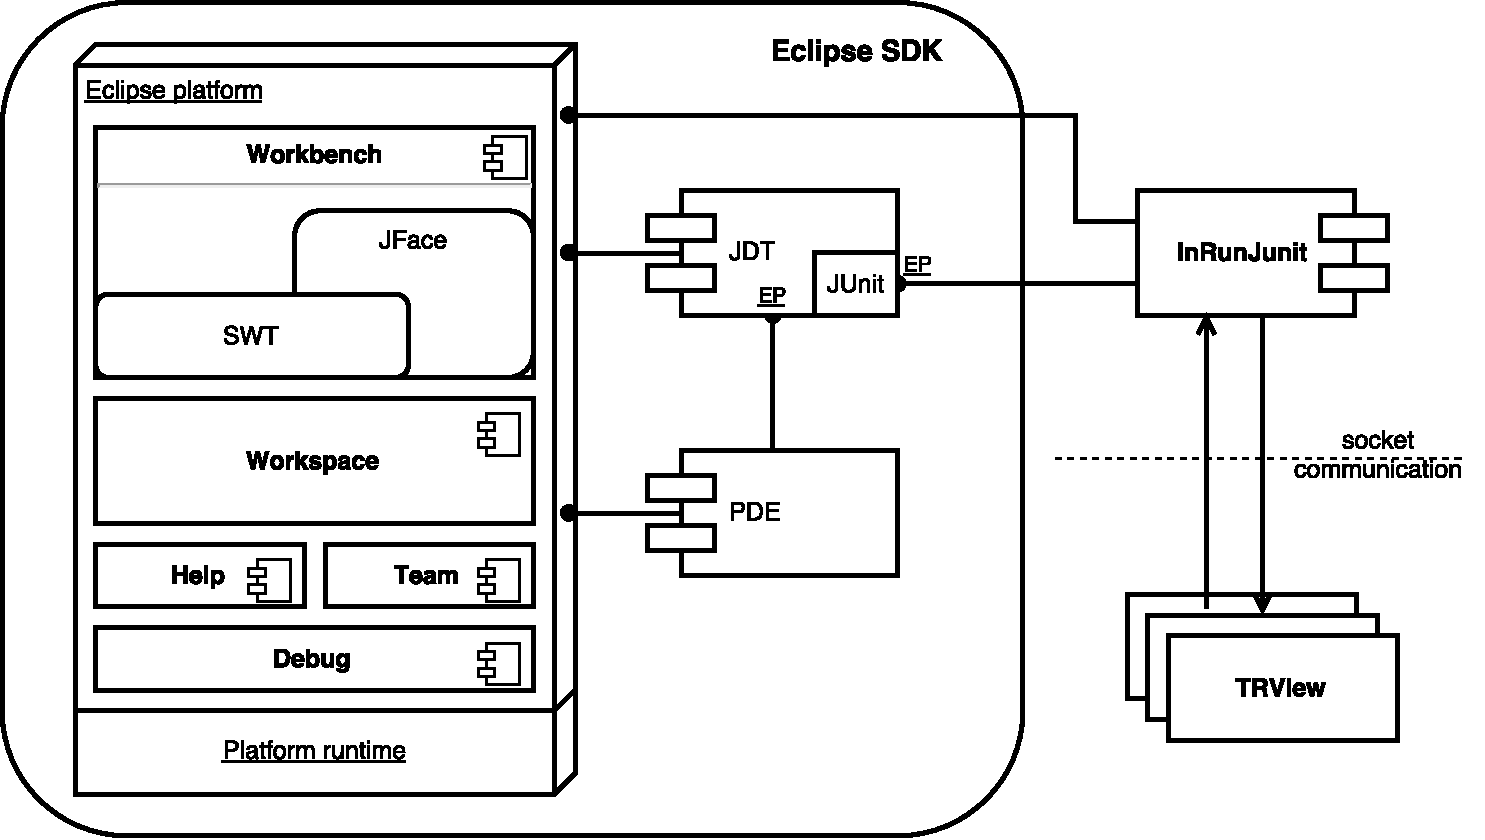
\includegraphics[width=\textwidth, center]{obrazky-figures/TRV_architecture.pdf}
    \caption{Znázornění architektury aplikace TRV.}
    \label{fig:TRV_architecture}
  \end{figure}

    \subsection{Návrh architektury zásuvného modulu InRunJUnit}
    Integrace zásuvného modulu InRunJUnit do platformy Eclipse je znázorněna na obrázku \ref{fig:inrunjunit_eclipse_integration}. Zásuvný modul se skládá ze dvou částí\,--\,\emph{listeneru} a serveru. Listener slouží pro zachycení výsledků ze zásuvného modulu JUnit. Opakem listeneru je potom \emph{notifier}, jehož účelem je informovat listener o nových datech. Listener je pomocí bodu rozšíření poskytovaného zásuvným modulem JUnit zaregistrován mezi ostatní listenery. Poté, co se spustí JUnit za účelem testování, si JUnit zjistí které zásuvné moduly jsou k bodu rozšíření připojeny a automaticky je informuje o průběhu testů. Server se stará o vytvoření serveru, komunikaci s klienty, vytvoření relevantních dat ve formě řetězce a jejich posílání všem připojeným klientům. Při posílání dat také specifikuje fázi testování\footnote{Může se jednat o zahájení (případně ukončení) testovací sady nebo testovacího případu.}, ze které data pochází.

      \begin{figure}[h]
	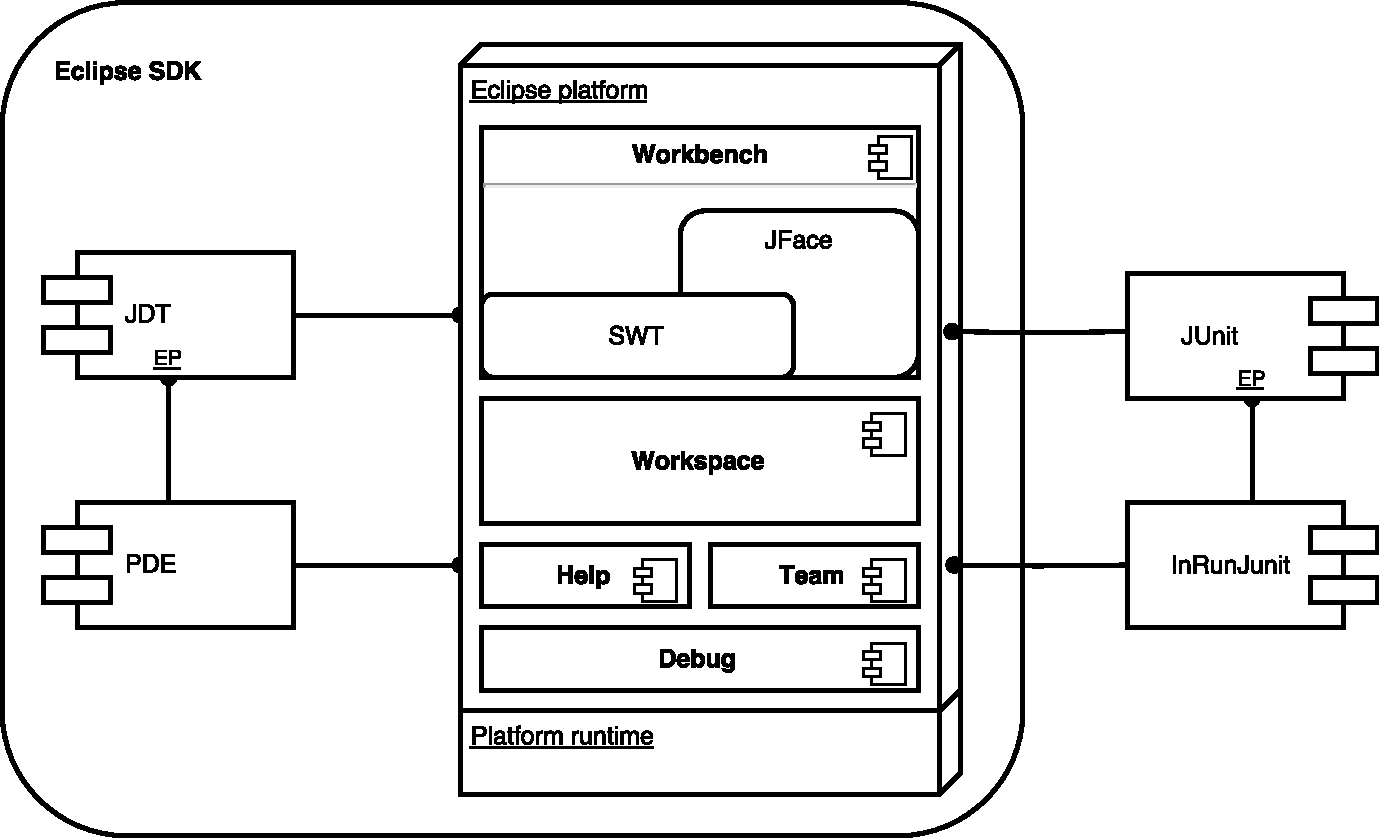
\includegraphics[width=\textwidth, center]{obrazky-figures/inrunjunit_eclipse_integration.pdf}
	\caption{Znázornění integrace zásuvného modulu InRunJUnit v platformě Eclipse.}
	\label{fig:inrunjunit_eclipse_integration}
      \end{figure}

    \subsection{Návrh architektury aplikace TRView}
    Aplikace TRView se také skládá ze dvou částí\,--\,klienta a GUI. Klientská část umožňuje připojení k serveru a ukládání přijatých výsledků. Při přijetí dat ze serveru také inicializuje zpracování a zobrazení průběhu testů do GUI. GUI se stará o vytvoření a obsluhu grafického uživatelského rozhraní\,--\,obsahuje komponenty sloužící pro připojení k serveru a zobrazuje důležité informace o průběhu testů. To zahrnuje:
    \begin{itemize}
     \item pole pro zadání adresy a portu serveru
     \item počet testovacích případů, které poběží
     \item počet testových chyb (\emph{angl. failures}) v testech
     \item počet běhových chyb (\emph{angl. errors}) v testech
     \item počet přeskočených testů
     \item stromovou strukturu jednotlivých testovacích případů s:
     \begin{itemize}
      \item rozlišením který test je aktivní
      \item rozlišením výsledku testovacího případu
      \item časem udávajícím trvání testovacího případu
     \end{itemize}
     \item zobrazení \emph{stack strace} pro neúspěšné testy
    \end{itemize}

    \noindent
    V případě, že testy a klientská aplikace poběží na jednom systému, je třeba vzít v úvahu problém aktivního okna. Některé testy vyžadují pro nalezení a otestování komponent aktivitu daného okna. To může způsobit překrytí okna aplikace TRView a tak znemožnit zobrazení informací o probíhajících testech uživateli. Proto je okno aplikace TRView vytvořeno \uv{vždy nahoře}(\emph{angl. always on top}). Okno je tak vždy viditelné, i když není právě aktivní.

    \subsection{Integrace zásuvného modulu InRunJUnit a SWT aplikace TRView}
    Komunikace mezi zásuvným modulem InRunJUnit a aplikací TRView je velmi důležitou částí návrhu. Ovlivňuje spoustu klíčových aspektů výsledné aplikace, které je třeba zvážit:
    \begin{itemize}
     \item rychlost komunikace
     \item možnost komunikace po síti
     \item počet možných klientů\,(instancí aplikace TRView) připojených k zásuvnému modulu InRUnJUnit
     \item oboustrannost komunikace
    \end{itemize}
    
    \noindent
    V aplikaci TRV je komunikace vyřešena pomocí klient-server modelu předávajícího informace pomocí soketů. Tento přístup poskytuje jednoduché a zároveň kompletní řešení uvedených problémů. Zpracováním dat v zásuvném modulu InRunJUnit lze posílat pouze relevantní data a tak minimalizovat objem posílaných dat a zrychlit komunikaci. Navíc tento model umožňuje připojení klientské aplikace po síti a řeší tak jednoduše problém s aktivitou oken. Díky paralelnímu programování lze připojit více klientských aplikací a zároveň umožnit oboustrannou komunikaci mezi všemi klienty a serverem. Oboustranná komunikace slouží k korektnímu ukončování jak serveru, tak klienta. V případě ukončení klienta je nutno oznámit serveru, že tomuto klientovi již nemá posílat data. V případě ukončení serveru je nutno oznámit všem klientům, že nemají čekat na další data. Oboustrannou komunikaci by však bylo možno využít i pro budoucí rozšíření, například pro kontrolu běhu testů z klientské aplikace.
    
    \begin{figure}[h]
      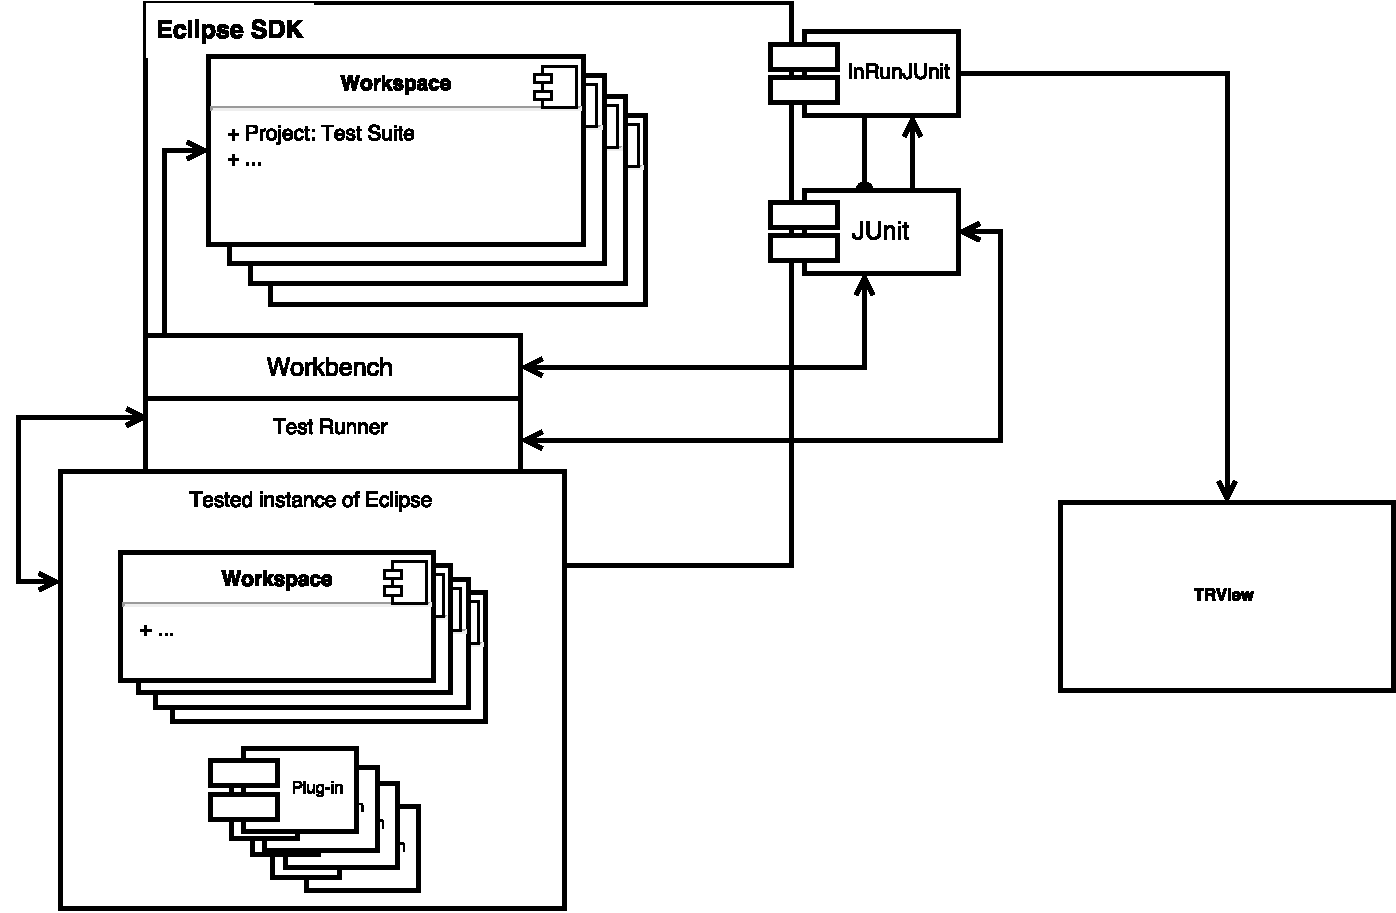
\includegraphics[width=\textwidth, center]{obrazky-figures/TRV_run_from_gui.pdf}
      \caption{Znázornění funkce aplikace TRV při spuštění testů z GUI Eclipse IDE.}
      \label{fig:TRV_run_from_gui}
    \end{figure}


  \section{Implementace aplikace TRV}
  %==================================
  Aplikace TRV je implementována v programovacím jazyce Java. Programovací jazyk Java byl vybrán na základě nutnosti implementace zásuvného modulu pro Eclipse IDE a následné komunikace s externí aplikací. Vývoj aplikace probíhá pomocí verze \emph{JavaSE-1.8} a je doporučeno tuto verzi pro další vývoj nebo testování používat.

    \subsection{Implementace zásuvného modulu InRunJUnit}
    Součástí implementace zásuvného modulu je vytvoření manifestů zásuvného modulu, implementace listeneru a implementace serverové části. Více o funkci manifestů a architektuře zásuvných modulů je uvedeno v kapitole \ref{chapter:eclipse_ide}.
      
      \subsubsection{Manifesty zásuvného modulu InRunJUnit}
	Manifesty zásuvného modulu slouží jako zdroj základních informací pro platformu Eclipse. V souboru \texttt{MANIFEST.MF} jsou data poskytující základní informace o daném modulu (viz obrázek \ref{code:manifest.mf}). Informace \texttt{Manifest-Version}, \texttt{Bundle-ManifestVersion}, \texttt{Bundle-Name}, \texttt{Bundle-SymbolicName}, \texttt{Bundle-Version} slouží pro popis manifestu a jednoznačnou identifikaci zásuvného modulu a z hlediska implementace nejsou příliš zajímavé. \texttt{Require-Bundle} obsahuje seznam všech ostatních balíčků, které jsou vyžadovány pro správné fungování zásuvného modulu. Za každým balíčkem může být ještě specifikována konkrétní verze balíčku, který je vyžadován. Balíčky uvedené na obrázku \ref{code:manifest.mf} slouží poskytují některé metody a třídy, které byly použity k implementaci listeneru a serveru. Poslední uvedený balíček\,--\,\texttt{org.jboss.reddeer.common}\,--\,je zde kvůli logování aplikace za účelem testování aplikace. \texttt{Bundle-RequiredExecutionEnvironment} specifikuje prostředí pro provádění aplikace\,--\,JavaSE verze 1.8. 
	
	\lstset{language=}
	\begin{figure}[h]
	  \begin{lstlisting}[frame=single]
Manifest-Version: 1.0
Bundle-ManifestVersion: 2
Bundle-Name: InRunJUnit
Bundle-SymbolicName: com.mcoufal.inrunjunit;singleton:=true
Bundle-Version: 1.0.0.qualifier
Require-Bundle: org.junit;bundle-version="4.12.0",
  org.eclipse.core.runtime;bundle-version="3.12.0",
  org.eclipse.debug.ui;bundle-version="3.11.201",
  org.eclipse.jdt.core;bundle-version="3.12.1",
  org.eclipse.jdt.junit.core,
  org.jboss.reddeer.common
Bundle-RequiredExecutionEnvironment: JavaSE-1.8
	  \end{lstlisting}
	  \caption{Zdrojový kód manifestu MANIFEST.MF obsahující základní informace o zásuvném modulu InRunJUnit.}
	  \label{code:manifest.mf}
	\end{figure}
	
	Manifest \texttt{plugin.xml} obsahuje pouze informaci, že třída \texttt{com.mcoufal.inrunjunit.listener.JUnitListenerEP} implementuje potřebné rozhraní pro bod rozšíření \texttt{org.eclipse.jdt.junit.testRunListeners} (viz obrázek \ref{code:plugin.xml}). Tato informace umožňuje, aby byl implementovaný listener načten a informován zásuvným modulem JUnit o průběhu testování. První dva řádky specifikují pouze verzi jazyka XML, ve kterém je manifest zapsán a verzi Eclipse IDE, ve které byl zásuvný modul vyvíjen.  

	\lstset{language=xml}
	\begin{figure}[h]
	  \begin{lstlisting}[frame=single]
<?xml version="1.0" encoding="UTF-8"?>
<?eclipse version="3.4"?>

<plugin>
  <extension point="org.eclipse.jdt.junit.testRunListeners">
    <testRunListener class="com.mcoufal.inrunjunit.listener.JUnitListenerEP"/>
  </extension>
</plugin>
	  \end{lstlisting}
	  \caption{Zdrojový kód manifestu plugin.xml zásuvného modulu InRunJunit.}
	  \label{code:plugin.xml}
	\end{figure}
     
      \subsubsection{Implementace listeneru}
	Balíček \texttt{listener} obsahuje pouze jednu třídu\,--\,\texttt{org.\-mcoufal.inrunjunit.listener.\\JUnitListenerEP}. Funkce této třídy je znázorněna na obrázku \ref{fig:listener_flowchart}. Instance třídy JUnitListenerEP je automaticky vytvořena zásuvným modulem JUnit, a to díky deklaraci připojení k bodu rozšíření \texttt{org.eclipse.jdt.junit.testRunListeners}. Při inicializaci si tato instance vytváří nový server, který je obsluhován dalším vláknem. Metody listeneru jsou poté volány pokaždé, když začne příslušná fáze v testování. To umožní při zavolání této metody zpracovat výsledky přijaté jako parametr dané metody a inicializovat jejich poslání pomocí dříve vytvořeného serveru. Pokud je zavolána metoda spojená s koncem testovací sady, je po předání výsledků serveru zároveň inicializováno jeho ukončení.
	
	Nejdůležitějším krokem implementace třídy \texttt{JUnitListenerEP} je rozšíření třídy \texttt{org.eclipse.jdt.junit.TestRunListener}. Přepsáním (\emph{angl. override}) metod této je dosaženo kontroly nad jednotlivými metodami, které rámec JUnit volá a tak informuje listener o průběhu testování.
	
	\begin{figure}[h]
	  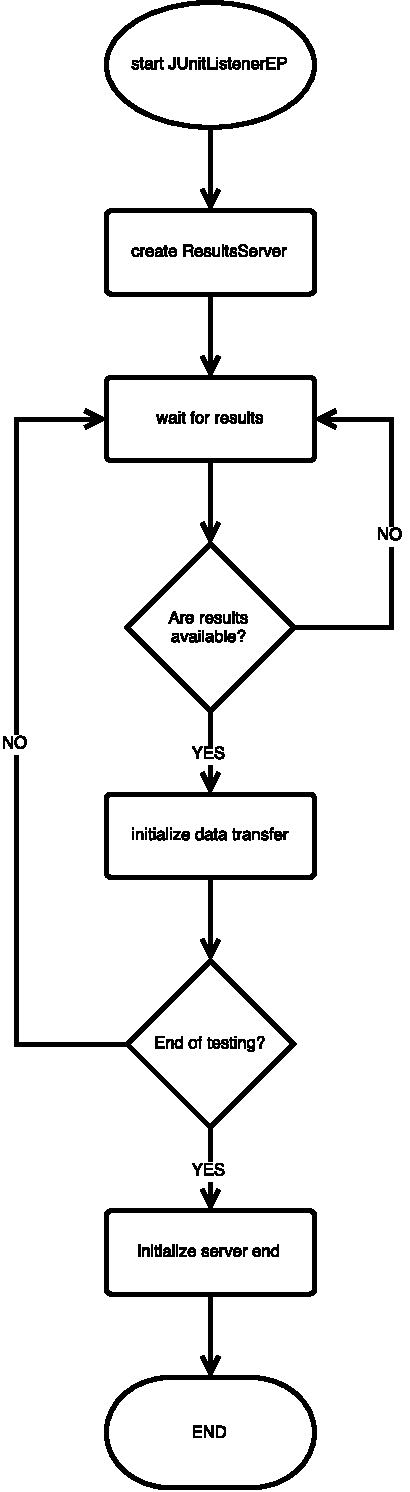
\includegraphics[width=\textwidth, height=0.8\textheight, keepaspectratio, center]{obrazky-figures/inrunjunit_listener_flowchart.pdf}
	  \caption{Diagram znázorňující funkci implementovaného listeneru \texttt{JUnitListenerEP} rozšiřujícího třídu \texttt{org.eclipse.jdt.junit.testRunListeners}.}
	  \label{fig:listener_flowchart}
	\end{figure}
      
      \subsubsection{Implementace serverové části}
	Hlavní třídou definující chování serveru je třída \texttt{ResultsServer} (viz obrázek \ref{fig:resultsserver_flowchart}). Tato třída má na starosti vytvoření serveru a správu klientů. Po vytvoření serveru na portu číslo 7357 se čeká na připojení klienta. Na každého připojeného klienta si ukládá odkaz a zároveň vytváří nové vlákno, které má na starosti obsluhu daného klienta. Tato obsluha je implementována ve třídě \texttt{ClientHandler}. Díky vytvořenému seznamu odkazů na jednotlivé klienty umožňuje třída \texttt{JUnitListenerEP} inicializovat posílání dat jednotlivým klientům a zároveň pomocí více vláken umožňuje obsluhu více klientů najednou. V případě zachycení dat spojených s ukončením testovací sady je po poslání dat server ukončen. Pro názornost je v diagramu na obrázku ukončení serveru zaznačeno, ve skutečnosti však ukončení serveru probíhá asynchronně.
	
	\begin{figure}[h]
	  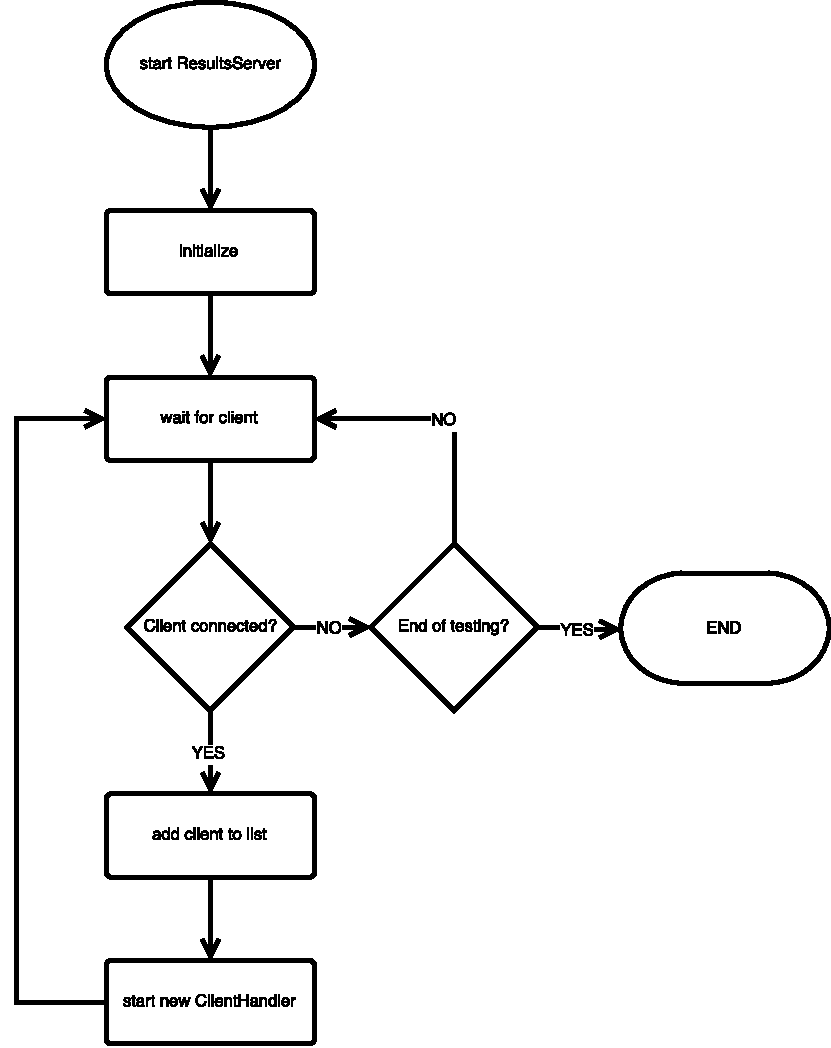
\includegraphics[width=\textwidth, center]{obrazky-figures/inrunjunit_resultsserver_flowchart.pdf}
	  \caption{Diagram znázorňující funkci implementovaného serveru \texttt{ResultsServer} zajišťujícího komunikaci mezi zásuvným modulem InRunJUnit a aplikací TRView.}
	  \label{fig:resultsserver_flowchart}
	\end{figure}

	Hlavním účelem třídy \texttt{ClientHandler} je obsluha klienta a přenos dat (viz Obrázek \ref{fig:clientHandler_flowchart}). Jakmile dojde k inicializaci a úspěšnému spojení s klientem, posílá se počáteční soubor dat. Tento soubor obsahuje všechna data zachycená pomocí listeneru do doby, než došlo k připojení klienta. Nedochází tak k ztrátě dat v případě, že se klient připojí až v průběhu testů. Dále se již posílají jen nově zachycená data (odesílání těchto dat inicializuje \texttt{JUnitListenerEP} prostřednictvím instance \texttt{ResultsServer}). Díky tomuto modelu komunikace nedochází k posílání irelevantních dat a zbytečnému zatížení síťové komunikace. \todo{Dopsat jak probíhá ukončení klienta}

	\begin{figure}[h]
	  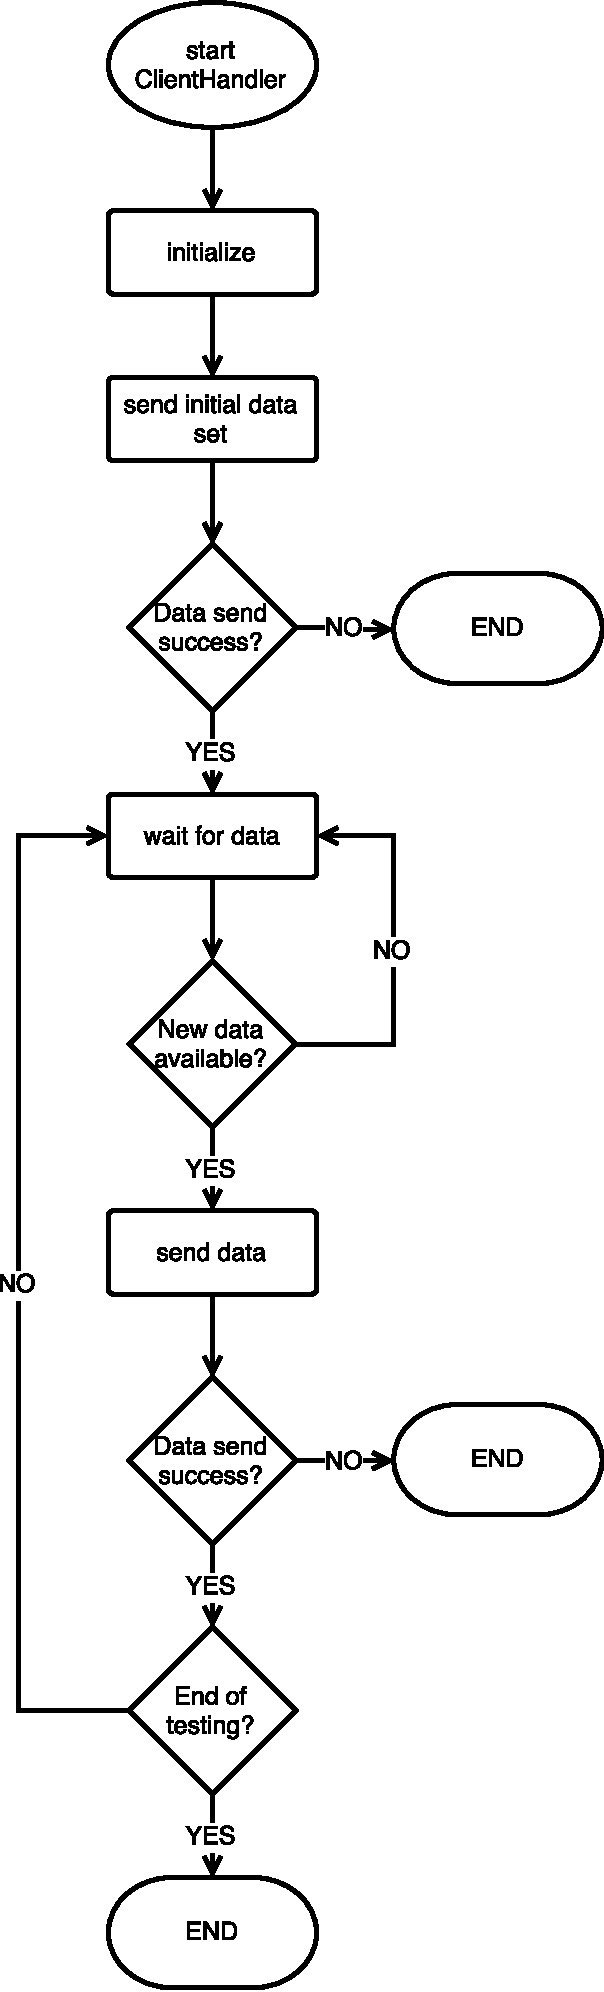
\includegraphics[width=\textwidth, height=0.9\textheight, keepaspectratio, center]{obrazky-figures/inrunjunit_clienthandler_flowchart.pdf}
	  \caption{Diagram znázorňující funkci obsluhy klienta implementovanou v třídě \texttt{ClientHandler}.}
	  \label{fig:clientHandler_flowchart}
	\end{figure}
	
	Dále serverová část obsahuje pouze třídy použité pro zpracování a posílání dat. Cílem těchto tříd je uložení potřebných informací do serializovatelné formy. Dosáhneme tak zmenšení objemu posílaných a jednoduššího zpracování dat v klientské aplikaci. Hlavní třídou pro manipulaci s výsledky je třída \texttt{ResultsData}. Ta obsahuje vždy instanci jednoho objektu a fázi, ve které byla data objektu zachycena. Díky fázi potom klient pozná, jak s objektem nakládat při zpracování a zobrazení dat. Ostatní třídy se starají pouze o uložení dat jednotlivých objektů do řetězcové nebo číselné podoby. Jedná se o třídy \texttt{StringDescription}, \texttt{StringResult}, \texttt{StringTestCaseElement}, \texttt{StringTestElement}, \texttt{StringTestRunSession}.

    \subsection{Implementace aplikace TRView}
    Implementace aplikace TRView je rozdělena do dvou balíčků\,--\,\texttt{view} a \texttt{client}. Balíček \texttt{view} zajišťuje vytvoření a obsluhu grafického uživatelského rozhraní a zároveň poskytuje metody pro zpracování a zobrazení dat získaných pomocí balíčku \texttt{client}. Balíček \texttt{client} se stará o komunikaci se serverem a inicializaci zobrazení dat uživateli. 
    
      \subsubsection{Implementace balíčku \texttt{view}}
      Balíček \texttt{view} obsahuje dvě třídy\,--\,\texttt{TRView} a \texttt{ResultsParser}. Třída \texttt{TRView} tvoří základ aplikace\,--\,inicializuje a vytváří grafické uživatelské rozhraní aplikace a definuje chování pro akce, které nastaly v GUI (akce provedené uživatelem pomocí myši nebo klávesnice). Pokud uživatel zadá IP adresu a port serveru, na kterém běží testy, stiskem tlačítka \texttt{CONNECT} se resetuje GUI, ukončí se instance stávajícího klienta \texttt{ResultsClient} (pokud byl již nějaký vytvořen) a vytvoří se nové vlákno zajišťující jeho funkci. V případě označení některého z testovacích případů se zobrazí jeho stack trace. Pokud uživatel ukončí aplikaci, inicializuje se konec klienta \texttt{ResultsClient} a aplikace se ukončí. Chování implementované v třídě TRView je znázorněno na obrázku \ref{fig:trview_flowchart}.\\
      
      \begin{figure}[h]
	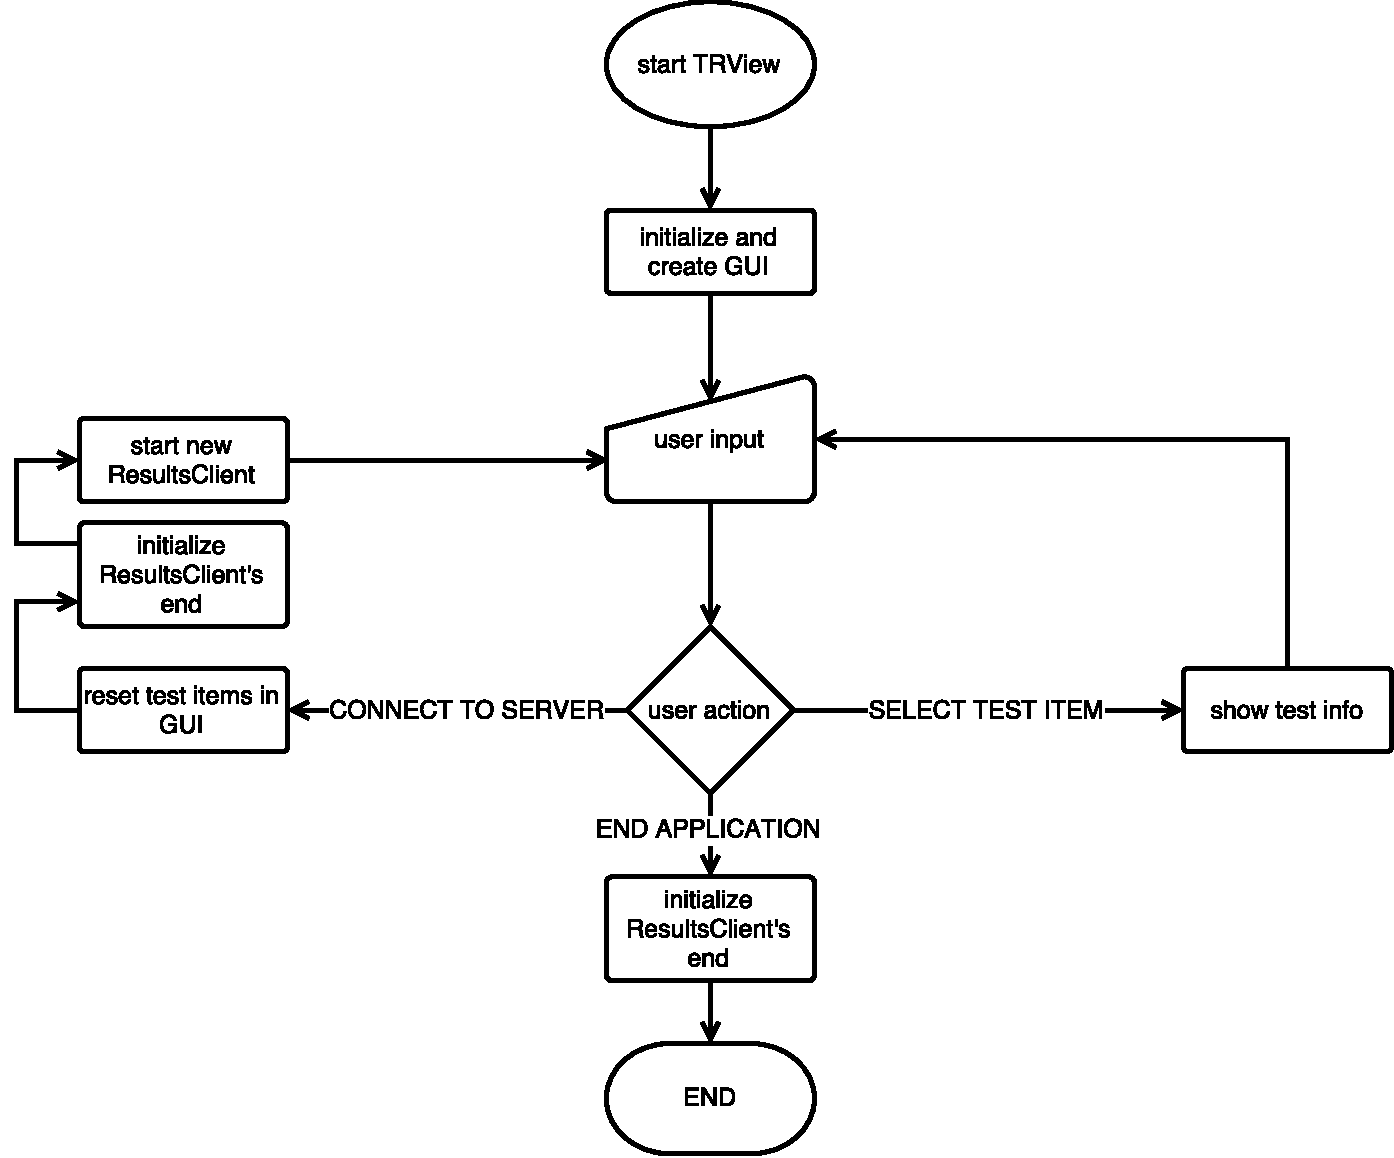
\includegraphics[width=\textwidth, height=\textheight, keepaspectratio, center]{obrazky-figures/trview_trview_flowchart.pdf}
	\caption{Diagram znázorňující funkci třídy TRView.}
	\label{fig:trview_flowchart}
      \end{figure}


      \noindent Grafické uživatelské rozhraní se skládá z:
      \begin{description}
	 \item[Menu] \todo{dodelat az bude implementace}
	 \item[Popisků:] slouží k identifikaci jednotlivých komponent (říkají tak uživateli, jaký je význam dat dané komponenty)
	 \item[Textových polí:] slouží pro zobrazení informací (počet chyb, běhů testů, atd.) nebo pro zadávání informací uživatelem (IP adresa serveru, port serveru).
	 \item[Stromová struktura:] je nejdůležitější část GUI aplikace. Do této struktury se zobrazuje průběh testů jednotlivých testovacích případů. Pro každý stav testovacího případu je zobrazena příslušná ikona (viz tabulka \ref{table:icons}) informující o stavu testu.
	 \item[Stack trace:] textový záznam zobrazující výpis metod které byly volány, než došlo u vybraného testovacího případu k chybě. Pokud žádná chyba nenastala, textové pole obsahuje pouze řetězec informující uživatele o tom, že stack trace je prázdný.
      \end{description}
      
      \todo{Popis ikon použitých v GUI - tabulka}
      %\begin{table}[h]
      % \begin{tabular}{c|c}
%	ikona & popis
%	ikona & popis
%	ikona & popis
%       \end{tabular}
%	\label{table:icons}
%	\caption{Použité ikony a jejich význam.}
%      \end{table}


      Třída \texttt{ResultsParser} obsahuje metody, které na vstupu zpracovávají instance třídy \texttt{ResultsData} a zobrazují je do GUI. Díky fázi uvedené v objektu \texttt{ResultsData} lze poznat, v jaké fázi testování byla data zachycena a podle toho data zpracovat a zobrazit. Jednotlivé fáze jsou definovány v třídě \texttt{JUnitListenerEP} zásuvného modulu InRunJunit.
      

      \subsubsection{Implementace balíčku \texttt{client}}
      Balíček \texttt{client} obsahuje pouze třídu \texttt{ResultsClient}. Funkce implementovaná touto třídou je znázorněna na obrázku \ref{fig:resultsclient_flowchart}. Instance třídy \texttt{ResultsClient} vzniká po zadání detailů připojení a stisku tlačítka \texttt{CONNECT} uživatelem. Instance se poté zkusí připojit k serveru na zadané IP adrese a portu. Pokud se připojení nezdaří, je uživateli vypsáno oznámení o chybě. Pokud proběhne připojení úspěšně, dochází k přijetí a zpracování počátečního souboru dat. Spojení mezi klientem a serverem je postaveno na spojované službě TCP a tak by nemělo docházet ke ztrátě dat. Pokud ovšem dojde k závažnějšímu problému na síti, je uživateli zobrazeno oznámení o chybě a \texttt{ResultsClient} je ukončen. Poté klient čeká na další data. Jakmile data obdrží, inicializuje jejich zpracování a zobrazení pomocí třídy \texttt{ResultsParser}. Jelikož upravujeme komponenty vytvořené jiným vláknem, je zapotřebí zajistit aby byl kód vykonán vláknem obsluhujícím GUI a nedocházelo tak k chybě typu \emph{Invalid Thread Access}. Proto je tato operaci prováděna pomocí synchronizace vláken (viz obrázek \ref{code:syncExec}). SWT poskytuje metodu syncExec(), která pozastaví průběh současného vlákna, a argument typu Runnable této metody předá vláknu obsluhujícího GUI. Jakmile je to možné, vlákno obsluhující GUI vykoná tento kód a dále pokračuje ve své práci. Po vykonání kódu je vlákno, ze kterého byla metoda syncExec() volána zase spuštěno \cite{codeaffine-asyncexec}. V případě zachycení dat s fází konce testovací sady se stejným způsobem inicializuje zpracování a zobrazení dat a poté se klient ukončí.
      
      \begin{figure}[h]
	  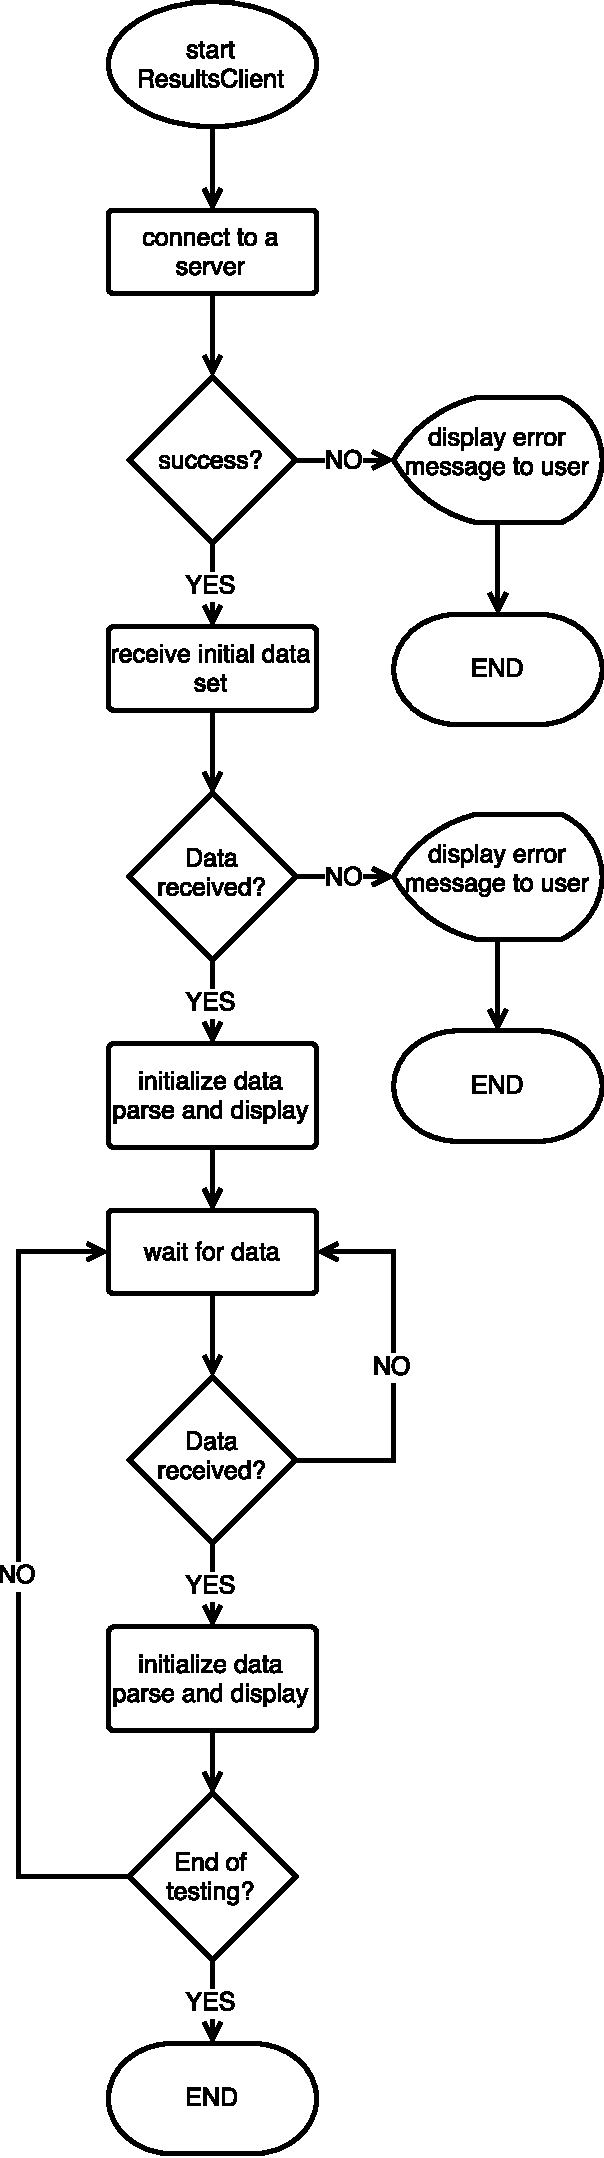
\includegraphics[width=\textwidth, height=0.95\textheight, keepaspectratio, center]{obrazky-figures/trview_resultsclient_flowchart.pdf}
	  \caption{Diagram znázorňující chování implementovaného klienta \texttt{ResultsClient.}}
	  \label{fig:resultsclient_flowchart}
	\end{figure}
      
      	\lstset{language=java}
	\begin{figure}[h]
	  \begin{lstlisting}[frame=single]
TRView.getDisplay().syncExec(new Runnable() {
	@Override
	public void run() {
		ResultsParser.parseAndDisplay(receivedData);
		TRView.redrawAllComponents();
	}
});
	  \end{lstlisting}
	  \caption{Zdrojový kód znázorňující práci s komponentami GUI z vlákna klienta \texttt{ResultsClient}. Metoda \texttt{parseAndDisplay(ResultsData)} zpracovává data a mění dle těchto dat GUI. Metoda \texttt{redrawAllComponents()} slouží k vykreslení všech komponent do GUI poté, co došlo ke změně komponenty.}
	  \label{code:syncExec}
	\end{figure}
      
      \todo{Az bude implementovano -- ukonceni klienta}
      
      
  \section{Testování}
  %==================
  Testování projektu proběhlo prozatím pouze manuálně -- byl vytvořen jeden projekt obsahující tři testovací sady. Testovací případy v každé sadě se zaměřují na jinou oblast. \todo{První testovací sada ... ipsum dolor sit amet.}

  \section{Praktické využití}
  %==========================
  Využití aplikace TRV spočívá především v použití při vývoji nebo opravách testů pro GUI platformy Eclipse. Spuštěním sady testů se otevře okno testované instance Eclipse IDE, kde probíhají jednotlivé testovací případy dané testovací sady. Bez pohledu JUnit však nelze jednoduše zjistit, který testovací případ právě běží a jak předchozí testovací případy dopadly.
  
  \todo{Co vse je treba mit nainstalovano? Staci jen Junita InRunJunit}
  Pro funkcionalitu aplikace TRV je nutno mít v Eclipse nainstalován zásuvné moduly JUnit a InRunJUnit. Na obrázku \ref{fig:TRV_run_from_gui} je znázorněno spuštění testovací sady z instance Eclipse IDE. Eclipse SDK představuje soubor všech komponent a zásuvných modulů, které Eclipse poskytuje jako minimální balíček pro vývoj aplikací. K tomuto minimálnímu balíčku lze instalovat další zásuvné moduly. V tomto případě se jedná o rámec JUnit a zásuvný modul InRunJunit. Uživatel vidí pouze Workbench, který mu umožňuje pracovat s jednotlivými projekty uloženýmy v pracovní ploše (Workspace). Spuštěním projektu s testovací sadou se uvědomí zásuvný modul JUnit a zvolený runner. Runner se stará o průběh testů a zároveň získává informace o průběhu testů. Tyto informace posílá zásuvnému modulu JUnit, který je dále zpracovává. Díky připojení pomocí bodů rozšíření může zásuvný modul JUnit automaticky informovat zásuvný modul InRunJUnit o průběhu testů. InRunJUnit tyto informace pomocí soketů posílá aplikaci TRView, která je zobrazuje na obrazovku.  
      
      \subsection{Instalace aplikace TRV}
      \todo{Lorem ipsum dolor sit amet.}

    \subsection{Použití při testování Eclipse IDE v~RedHat}
    %**************************************************
    Testování Eclipse IDE probíhá z velké části automatizovaně. Testovací sady jsou spouštěny oproti jednotlivým verzím operačního systému RHEL a Eclipse IDE. Tyto testy jsou spouštěny buď manuálně, nebo po splnění nastavených podmínek pomocí serveru Jenkins\todo{footnote}. Testy jsou spuštěny přímo z konzole a nevzniká tak druhé okno s GUI Eclipse IDE. Testování probíhá na vybraných serverech, které jsou vybrány dle potřeby testera.
    
    \todo{Kod - priklad spousteni testu z konzole}
    \lstset{language=bash}
    \begin{figure}[h]
	  \begin{lstlisting}[frame=single]
echo "TODO:"
	  \end{lstlisting}
	  \caption{TODO:}
	  \label{code:syncExec}
	\end{figure}
    
    \todo{Popis obrazku}

    \begin{figure}[h]
	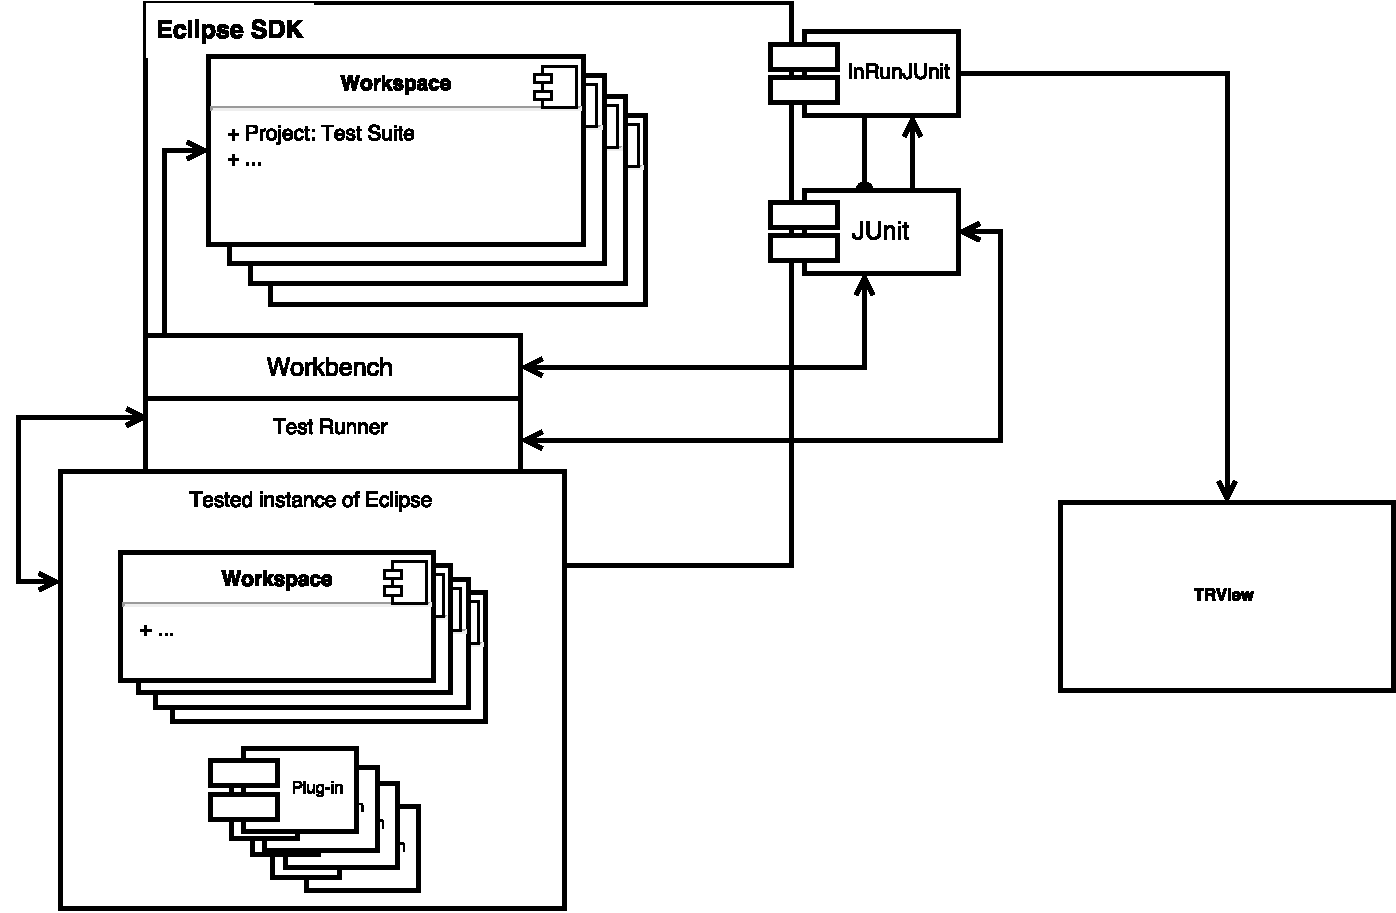
\includegraphics[width=\textwidth, center]{obrazky-figures/TRV_run_from_term.pdf}
	\caption{Znázorňění funkce aplikace TRV při spuštění testů z terminálu.}
	\label{fig:TRV_run_from_term}
      \end{figure}

  \section{Další rozšíření}
  %========================
  Díky obousměrné komunikaci mezi klientskou a serverovou částí má aplikace TRV potenciál na mnohá rozšíření. Užitečnou funkcionalitou by bylo například pozastavení průběhu testů. Uživatel by tak mohl mezitím lépe prozkoumat příčinu neúspěšného testu nebo uvést testovanou instanci do korektního stavu\footnote{Aby nedošlo k zbytečnému selhání následujících testovacích případů.}. \todo{rozsireni-to co poskytuje JUnit}
  
  \todo{Pokud nejakou funkcionalitu nestihnu - je vhodne ji tady zminit}
  %=========================================================================%
% - - - KAPITOLA 5: Z Á V Ě R                                             %
\chapter{Závěr}                                                           %
%=========================================================================%
Tato práce se zabývá návrhem a implementací nástrojů poskytujících informace o~probíhajících testech uživatelského rozhraní platformy Eclipse. Tyto nástroje  jsou navrženy pro funkci s~testovacím rámcem JUnit, obsaženým v~Eclipse JDT (Java Development Tools). V~první části je popsána architektura platformy Eclipse, se zaměřením na strukturu a tvorbu zásuvných modulů. Druhá část se zabývá architekturou testovacího rámce JUnit, jeho aplikačním rozhraním, možnostmi rozšíření a jeho integrací ve vývojovém prostředí Eclipse.

Hlavní část práce představuje autorem implementovaný nástroj TRV, skládající se ze dvou částí\,--\,InRunJUnit a TRView. Díky těmto nástrojům lze sledovat průběh testů uživatelského rozhraní, bez problémů s~aktivitou okna. Uživateli je zobrazena stromová struktura s~vyznačenými stavy jednotlivých testovacích případů. Zároveň poskytuje uživateli přehled o~počtu běhů testů, testových chyb, běhových chyb a ignorovaných testovacích případů. V~případě chybného testovacího případu zobrazuje i výpis posledních volání na zásobníku (angl. stack trace).

Nástroj TRV byl předán firmě Red Hat, kde bude diskutována a navržena jeho modifikace pro budoucí použití. \todo{...Zjistit jaké jsou plány s~projektem...}

  % Pouzita literatura / Bibliography
  % ----------------------------------------------
\ifslovak
  \makeatletter
  \def\@openbib@code{\addcontentsline{toc}{chapter}{Literatúra}}
  \makeatother
  \bibliographystyle{bib-styles/czechiso}
\else
  \ifczech
    \makeatletter
    \def\@openbib@code{\addcontentsline{toc}{chapter}{Literatura}}
    \makeatother
    \bibliographystyle{bib-styles/czechiso}
  \else 
    \makeatletter
    \def\@openbib@code{\addcontentsline{toc}{chapter}{Bibliography}}
    \makeatother
    \bibliographystyle{bib-styles/englishiso}
  %  \bibliographystyle{alpha}
  \fi
\fi
  \begin{flushleft}
  \bibliography{xcoufa08-Pohled-na-stav-JUnit-pro-testovanou-instanci-eclipse-20-literatura-bibliography}
  \end{flushleft}

  % vynechani stranky v oboustrannem rezimu
  % Skip the page in the two-sided mode
  \iftwoside
    \cleardoublepage
  \fi

  % Prilohy / Appendices TODO: Uncomment appendix, appendixpage, startcontents[chapter] if appendices pressent
  % ---------------------------------------------
  %\appendix
\ifczech
  \renewcommand{\appendixpagename}{Přílohy}
  \renewcommand{\appendixtocname}{Přílohy}
  \renewcommand{\appendixname}{Příloha}
\fi
\ifslovak
  \renewcommand{\appendixpagename}{Prílohy}
  \renewcommand{\appendixtocname}{Prílohy}
  \renewcommand{\appendixname}{Príloha}
\fi
  %\appendixpage

% vynechani stranky v oboustrannem rezimu
% Skip the page in the two-sided mode
\iftwoside
  \cleardoublepage
\fi
  
\ifslovak
%  \section*{Zoznam príloh}
%  \addcontentsline{toc}{section}{Zoznam príloh}
\else
  \ifczech
%    \section*{Seznam příloh}
%    \addcontentsline{toc}{section}{Seznam příloh}
  \else
%    \section*{List of Appendices}
%    \addcontentsline{toc}{section}{List of Appendices}
  \fi
\fi
  %\startcontents[chapters]
  % seznam příloh / list of appendices
  % \printcontents[chapters]{l}{0}{\setcounter{tocdepth}{2}}
  
  % vynechani stranky v oboustrannem rezimu
  \iftwoside
    \cleardoublepage
  \fi
  %\chapter{Obsah přiloženého paměťového média}
\label{jak}

\begin{itemize}
 \item {\LARGE \textbf{TRV/:} kořenový adresář.}
    {\Large \begin{itemize}
     \item \textbf{mcoufal.InRunJUnit:}
	Adresář obsahující zdrojové soubory implementovaného zásuvného modulu InRunJUnit.
     \item \textbf{mcoufal.InRunJUnit.feature:}
	Adresář obsahující feature projekt se zásuvným modulem InRunJUnit.
     \item \textbf{mcoufal.InRunJUnit.updateSite:}
	Adresář obsahující update site projekt se zásuvným modulem InRunJUnit.
     \item \textbf{README.md:}
	Soubor popisující základní použití a instalaci vytvořeného nástroje TRV.
     \item \textbf{technical-report:}
	Adresář obsahující zdrojové soubory použité pro tvorbu této práce.
     \item \textbf{TRView:}
	Adresář obsahující zdrojové soubory aplikace TRView a spustitelný JAR archiv \texttt{TRView.jar}.
     \item \textbf{xcoufa08-Pohled-na-stav-JUnit-pro-testovanou-instanci-eclipse.pdf:}
	Soubor ve formátu PDF obsahující elektronickou verzi této práce.
    \end{itemize}}
\end{itemize}


 % viz. prilohy.tex / see prilohy.tex TODO: uncomment if any appendices pressent
\end{document}
